\section{Erlang Observer
可视化入门}\label{erlang-observer-ux53efux89c6ux5316ux5165ux95e8}

\begin{quote}
本文介绍 Erlang/OTP 自带的图形化观察工具
Observer。它的价值不是``多一个监控面板''，而是让我们直接看见正在运行的
BEAM 节点：application、supervisor tree、worker
process、消息队列、进程状态、内存和调度器信息。
\end{quote}

\begin{center}\rule{0.5\linewidth}{0.5pt}\end{center}

\subsection{1. 为什么先讲
Observer}\label{ux4e3aux4ec0ux4e48ux5148ux8bb2-observer}

学习 OTP 时，如果直接从
\texttt{application}、\texttt{supervisor}、\texttt{gen\_server}、\texttt{gen\_statem}
的回调函数开始，很容易把 OTP 学成一堆 API。

Observer 提供了另一种学习方式：

\begin{Shaded}
\begin{Highlighting}[]
\NormalTok{先启动一个真实 OTP 应用}
\NormalTok{  {-}\textgreater{} 用 Observer 看见 application}
\NormalTok{  {-}\textgreater{} 展开 supervision tree}
\NormalTok{  {-}\textgreater{} 找到 supervisor 和 worker process}
\NormalTok{  {-}\textgreater{} 双击进程查看 Process Information / State}
\NormalTok{  {-}\textgreater{} 再回到代码理解 behaviour callback}
\end{Highlighting}
\end{Shaded}

这条路线更适合自顶向下理解 OTP。

在本教程中，我们使用 \texttt{full\_otp\_app} 作为演示项目。它包含：

\begin{Shaded}
\begin{Highlighting}[]
\NormalTok{full\_otp\_app (application)}
\NormalTok{  └── full\_otp\_app\_sup (supervisor, one\_for\_one)}
\NormalTok{      ├── kv\_server      (gen\_server)}
\NormalTok{      ├── event\_bus      (gen\_event)}
\NormalTok{      ├── traffic\_light  (gen\_statem)}
\NormalTok{      └── data\_store\_sup (supervisor, rest\_for\_one)}
\NormalTok{          ├── data\_store (gen\_server, DETS)}
\NormalTok{          └── data\_cache (gen\_server, ETS cache)}
\end{Highlighting}
\end{Shaded}

对应源码位于：

\begin{itemize}
\tightlist
\item
  \texttt{full\_otp\_app/src/full\_otp\_app.app.src}
\item
  \texttt{full\_otp\_app/src/full\_otp\_app\_sup.erl}
\item
  \texttt{full\_otp\_app/src/kv\_server.erl}
\item
  \texttt{full\_otp\_app/src/traffic\_light.erl}
\item
  \texttt{full\_otp\_app/src/data\_store\_sup.erl}
\end{itemize}

\begin{center}\rule{0.5\linewidth}{0.5pt}\end{center}

\subsection{2. 启动 demo 应用和
Observer}\label{ux542fux52a8-demo-ux5e94ux7528ux548c-observer}

进入 demo 项目：

\begin{Shaded}
\begin{Highlighting}[]
\BuiltInTok{cd}\NormalTok{ bilibili\_erlang/observer/full\_otp\_app}
\ExtensionTok{rebar3}\NormalTok{ shell }\AttributeTok{{-}{-}sname}\NormalTok{ application\_demo}
\end{Highlighting}
\end{Shaded}

如果 application 没有自动启动，可以在 Erlang shell 中执行：

\begin{Shaded}
\begin{Highlighting}[]
\FunctionTok{application:ensure\_all\_started(}\CharTok{full\_otp\_app}\FunctionTok{).}
\end{Highlighting}
\end{Shaded}

启动 Observer：

\begin{Shaded}
\begin{Highlighting}[]
\FunctionTok{observer:start().}
\end{Highlighting}
\end{Shaded}

启动后可以看到 Observer 图形窗口。

\begin{figure}
\centering
\pandocbounded{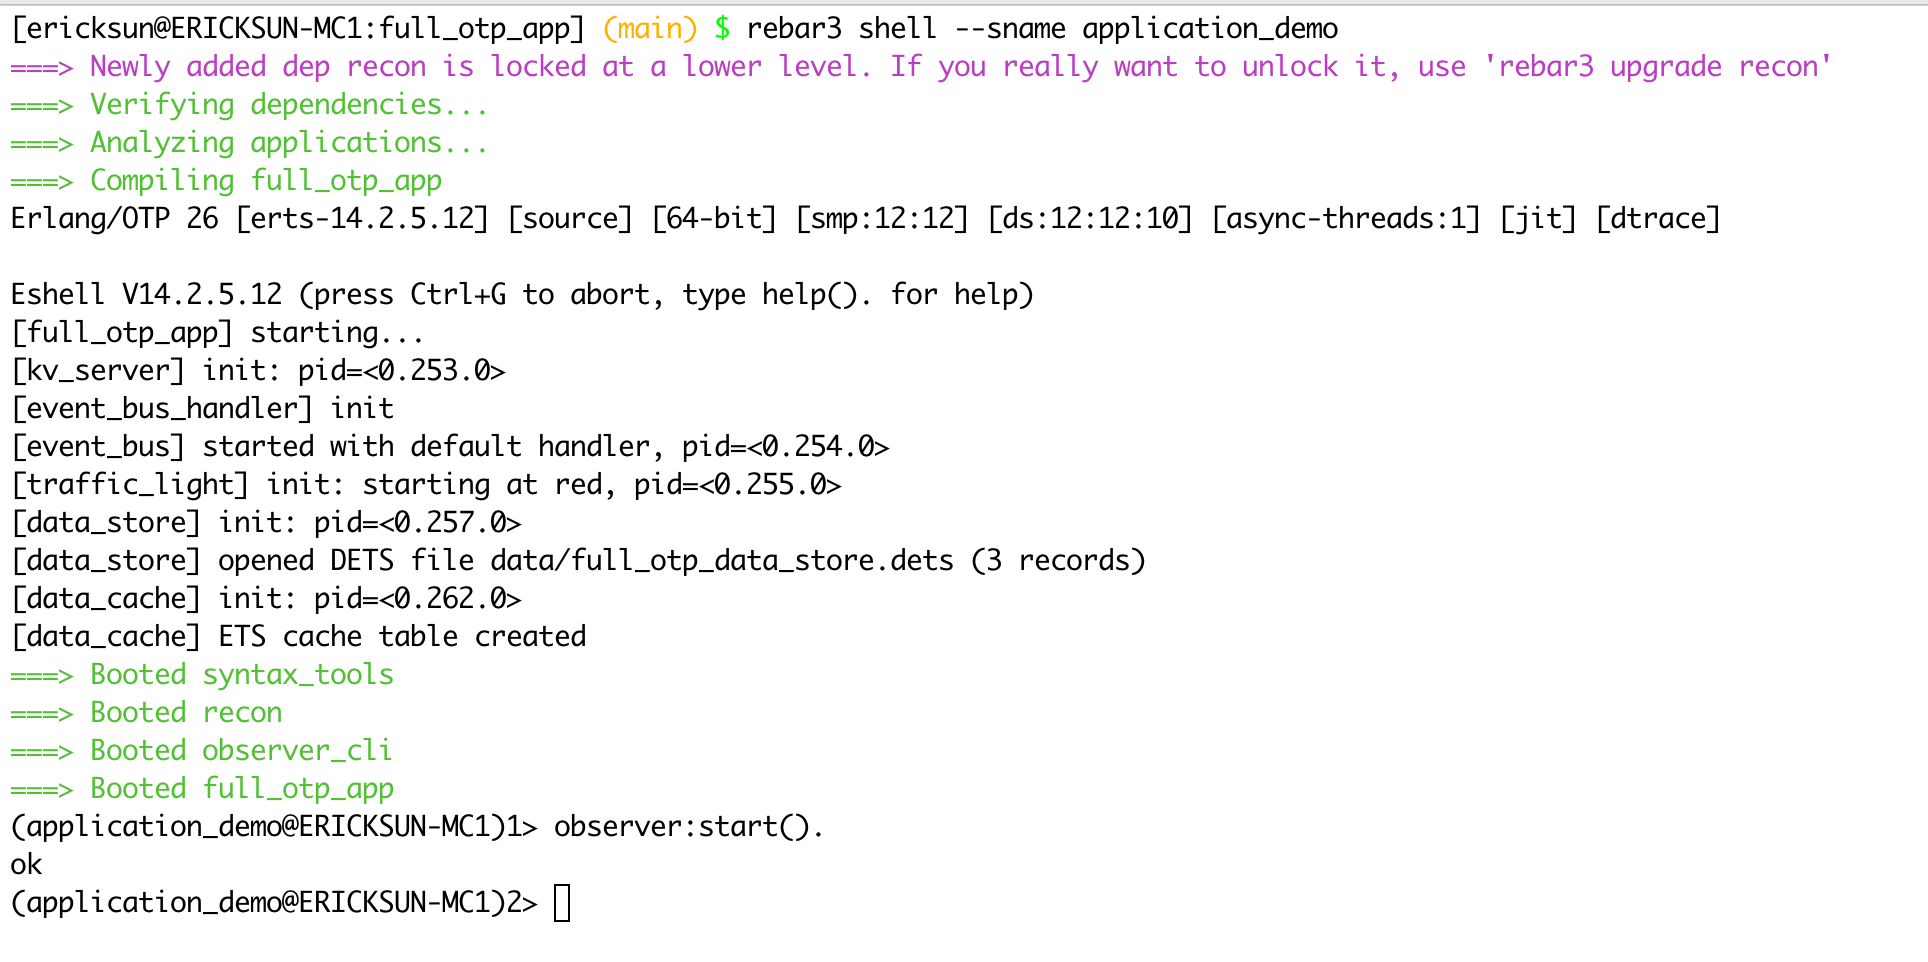
\includegraphics[keepaspectratio]{images/observer_start.png}}
\caption{启动 Observer}
\end{figure}

这一张图适合作为课程开场：左侧是 Erlang shell，右侧是 Observer
图形界面。它传达的重点是：Observer 不是外部猜测工具，而是连接到当前 BEAM
节点，直接查看运行时内部结构。

\begin{center}\rule{0.5\linewidth}{0.5pt}\end{center}

\subsection{3.
System：先看节点整体状态}\label{systemux5148ux770bux8282ux70b9ux6574ux4f53ux72b6ux6001}

Observer 打开后，默认可以先看 \texttt{System} 页面。

\begin{figure}
\centering
\pandocbounded{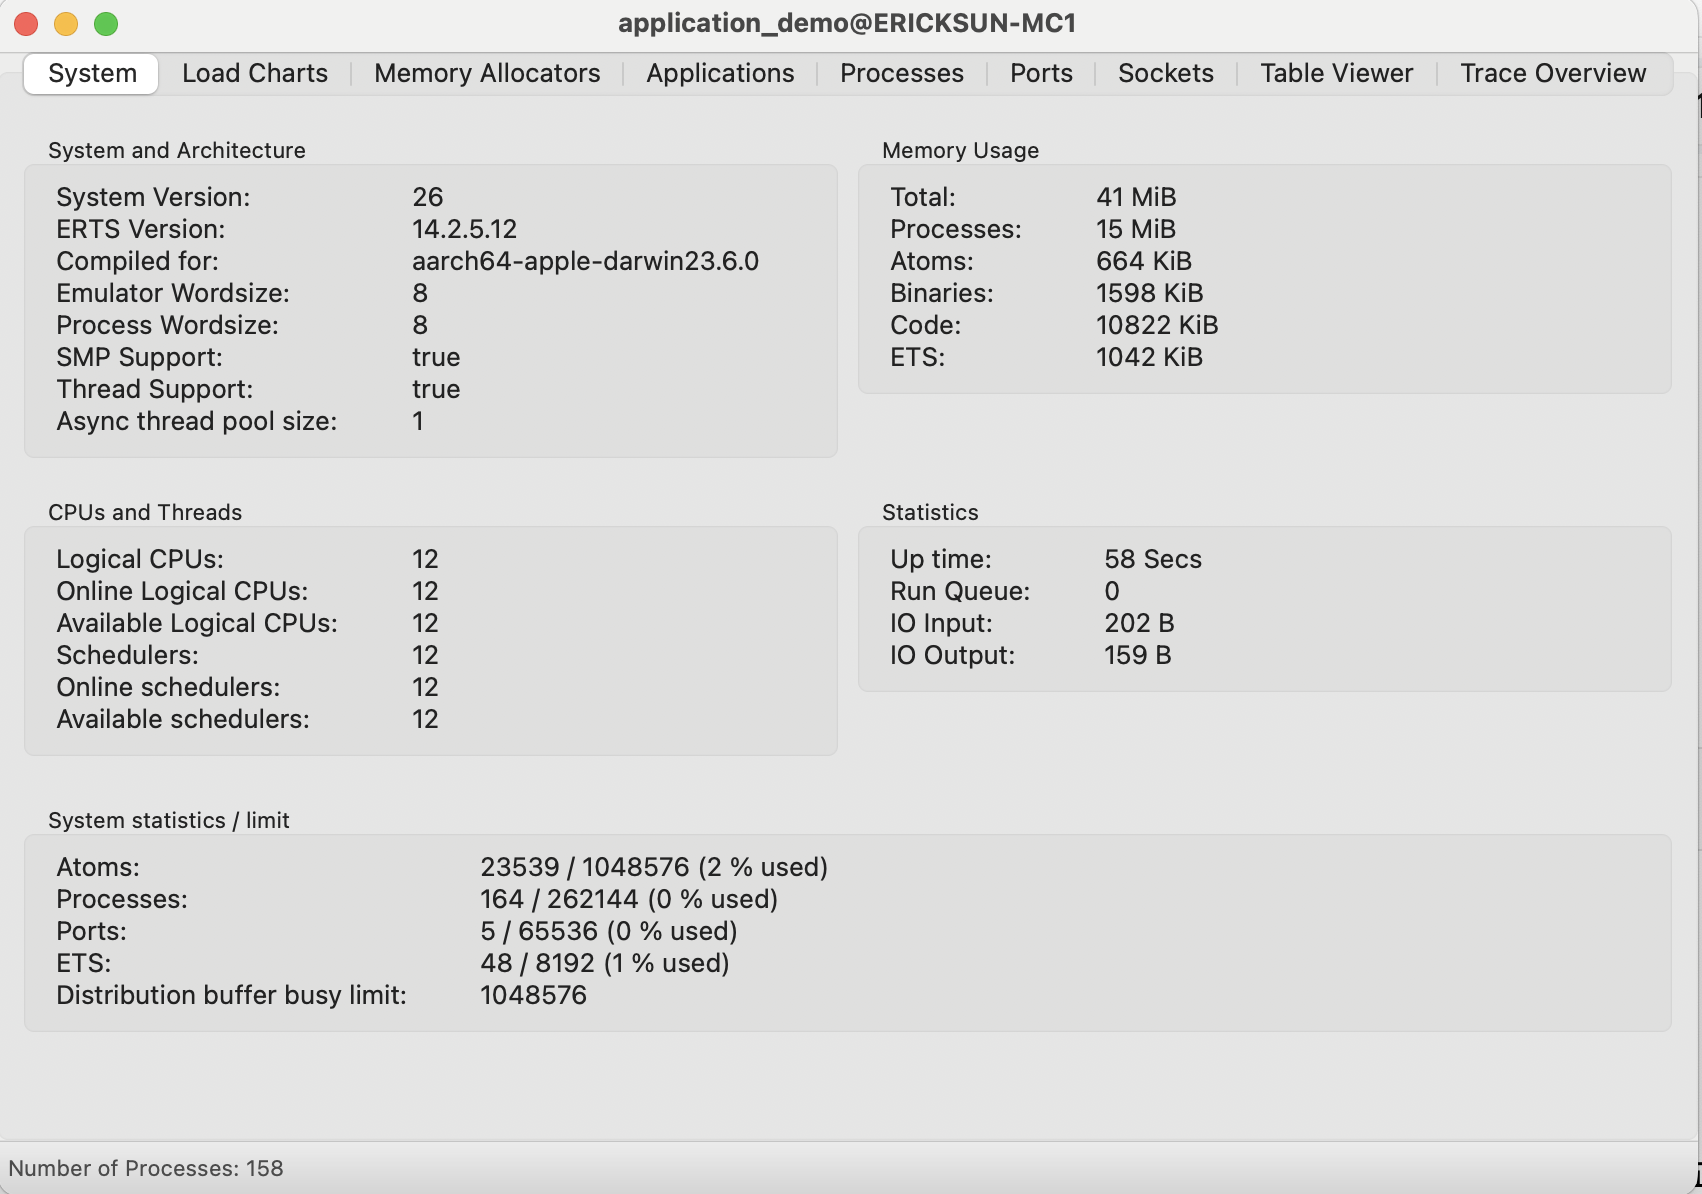
\includegraphics[keepaspectratio]{images/System.png}}
\caption{System 页面}
\end{figure}

\texttt{System} 页面适合建立第一层印象：

\begin{itemize}
\tightlist
\item
  当前节点名称。
\item
  OTP 版本和系统信息。
\item
  进程数量。
\item
  内存使用情况。
\item
  scheduler 信息。
\item
  atom、port、ETS、timer 等运行时资源。
\end{itemize}

这一页不需要讲得很细。对初学者来说，只要记住：Erlang
节点不是一个黑盒进程，BEAM VM 内部的资源都可以被观察。

\begin{center}\rule{0.5\linewidth}{0.5pt}\end{center}

\subsection{4. Load
Charts：观察运行时负载}\label{load-chartsux89c2ux5bdfux8fd0ux884cux65f6ux8d1fux8f7d}

\texttt{Load\ Charts} 页面展示节点运行时的负载曲线。

\begin{figure}
\centering
\pandocbounded{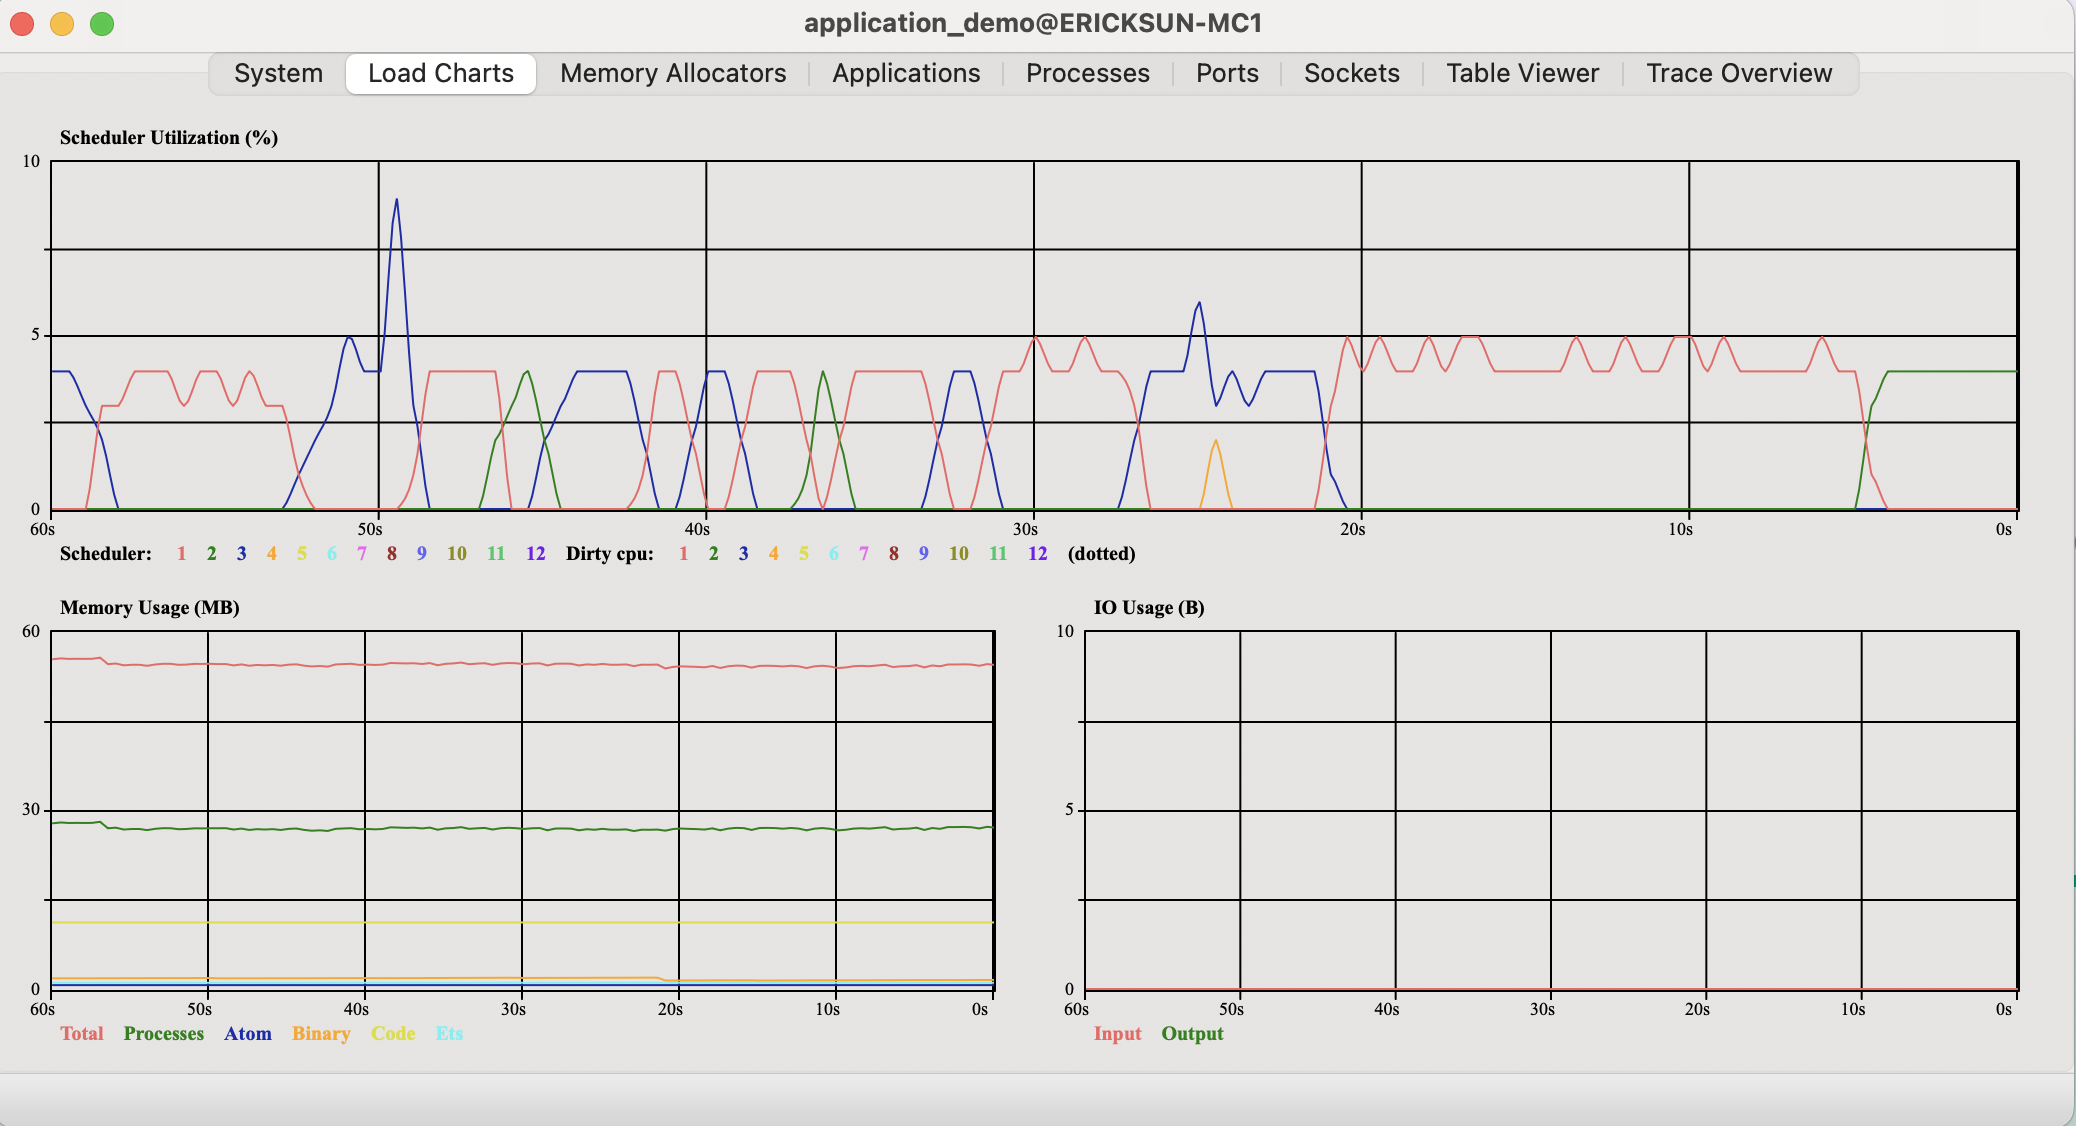
\includegraphics[keepaspectratio]{images/Load_Charts.png}}
\caption{Load Charts 页面}
\end{figure}

这里可以介绍几个概念：

\begin{longtable}[]{@{}ll@{}}
\toprule\noalign{}
指标 & 说明 \\
\midrule\noalign{}
\endhead
\bottomrule\noalign{}
\endlastfoot
Scheduler Utilization & scheduler 使用率，反映 BEAM 调度器是否繁忙 \\
Run Queue & 等待运行的 Erlang process 数量 \\
IO & 输入输出相关负载 \\
Memory & 内存变化趋势 \\
\end{longtable}

这一页可以用来说明：Erlang 的并发不是 OS thread 级别的手工调度，而是
BEAM 调度大量轻量级 Erlang process。

\begin{center}\rule{0.5\linewidth}{0.5pt}\end{center}

\subsection{5. Memory
Allocators：观察内存分配器}\label{memory-allocatorsux89c2ux5bdfux5185ux5b58ux5206ux914dux5668}

\texttt{Memory\ Allocators} 页面展示不同 allocator 的内存使用情况。

\begin{figure}
\centering
\pandocbounded{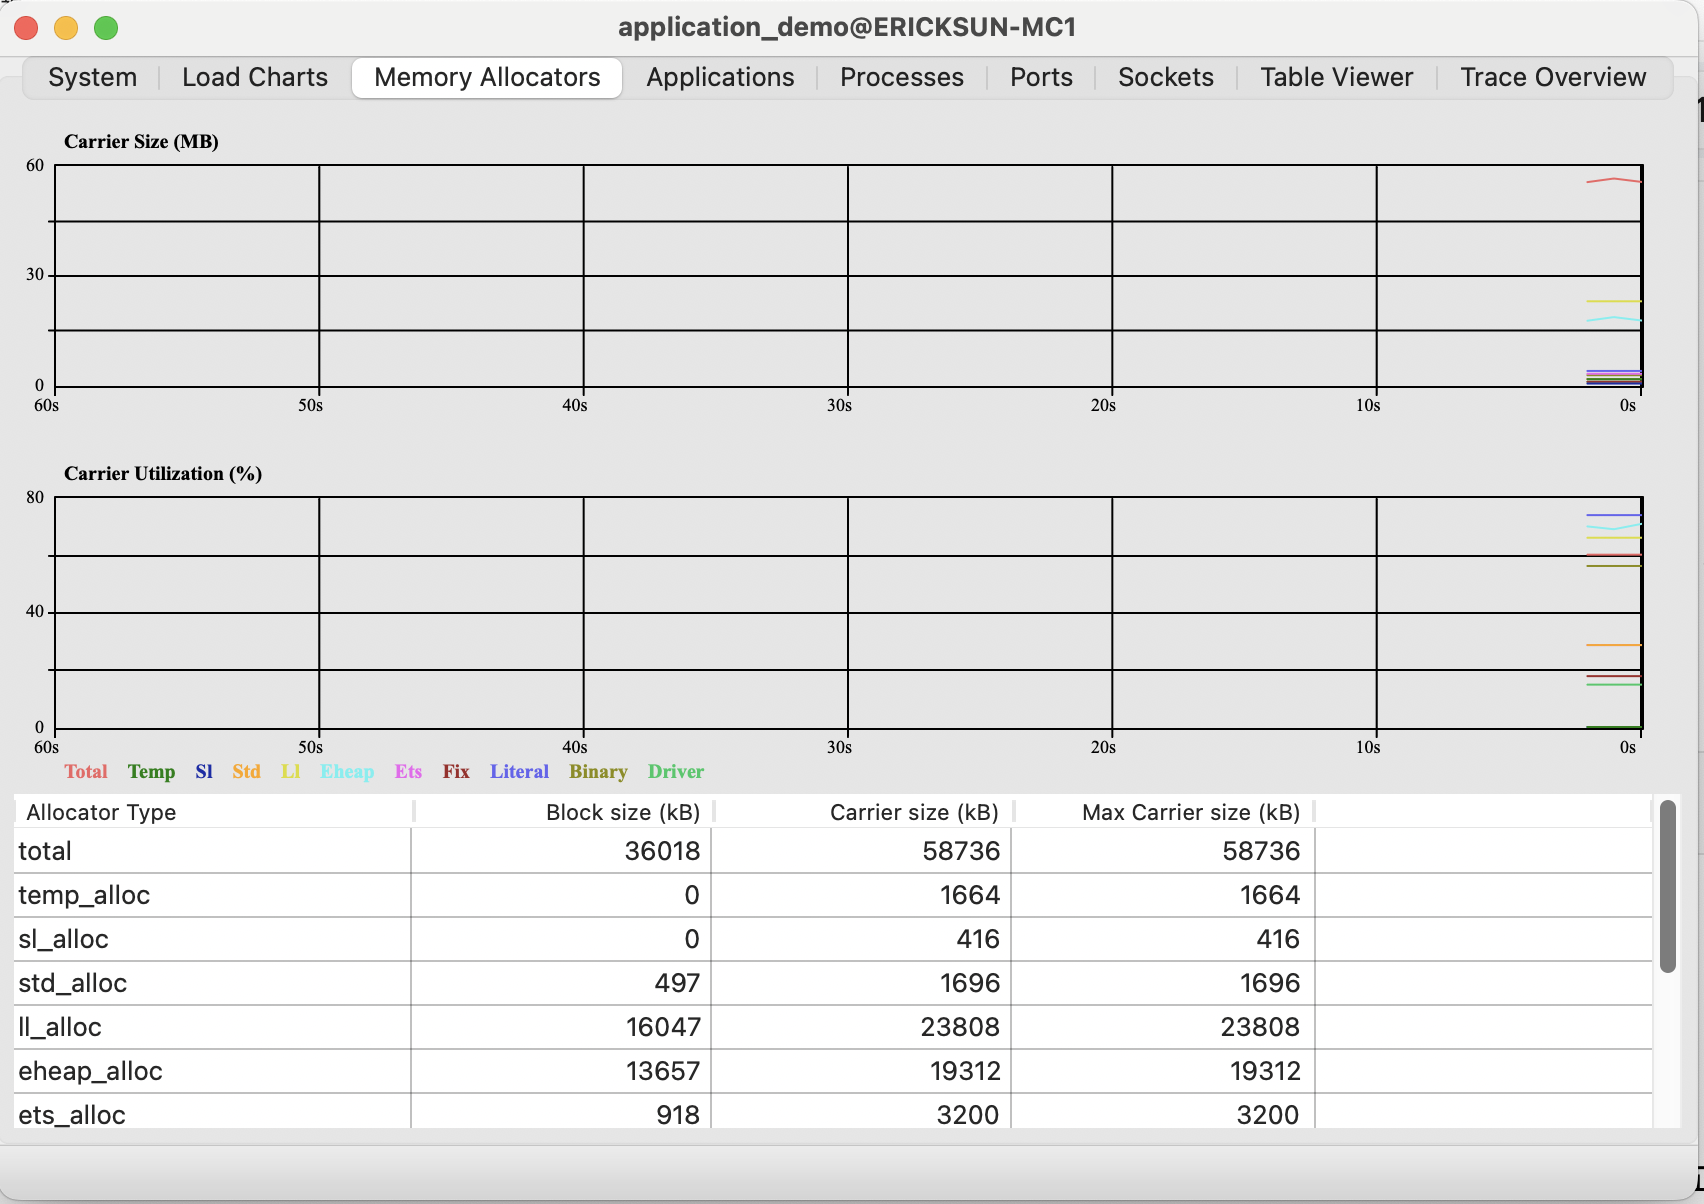
\includegraphics[keepaspectratio]{images/Memory_Allocators.png}}
\caption{Memory Allocators 页面}
\end{figure}

这部分对入门课不需要展开太深。建议只讲两个点：

\begin{enumerate}
\def\labelenumi{\arabic{enumi}.}
\tightlist
\item
  BEAM 的内存不是一个简单总数，内部有不同 allocator。
\item
  真正做性能诊断时，Observer 可以帮助定位内存增长来自哪里。
\end{enumerate}

如果课程重点是 OTP，可以快速带过这一页，把主要时间留给
\texttt{Applications} 和 \texttt{Processes}。

\begin{center}\rule{0.5\linewidth}{0.5pt}\end{center}

\subsection{6. Applications：从 application 开始理解
OTP}\label{applicationsux4ece-application-ux5f00ux59cbux7406ux89e3-otp}

\texttt{Applications} 页面是本教程的核心。

\begin{figure}
\centering
\pandocbounded{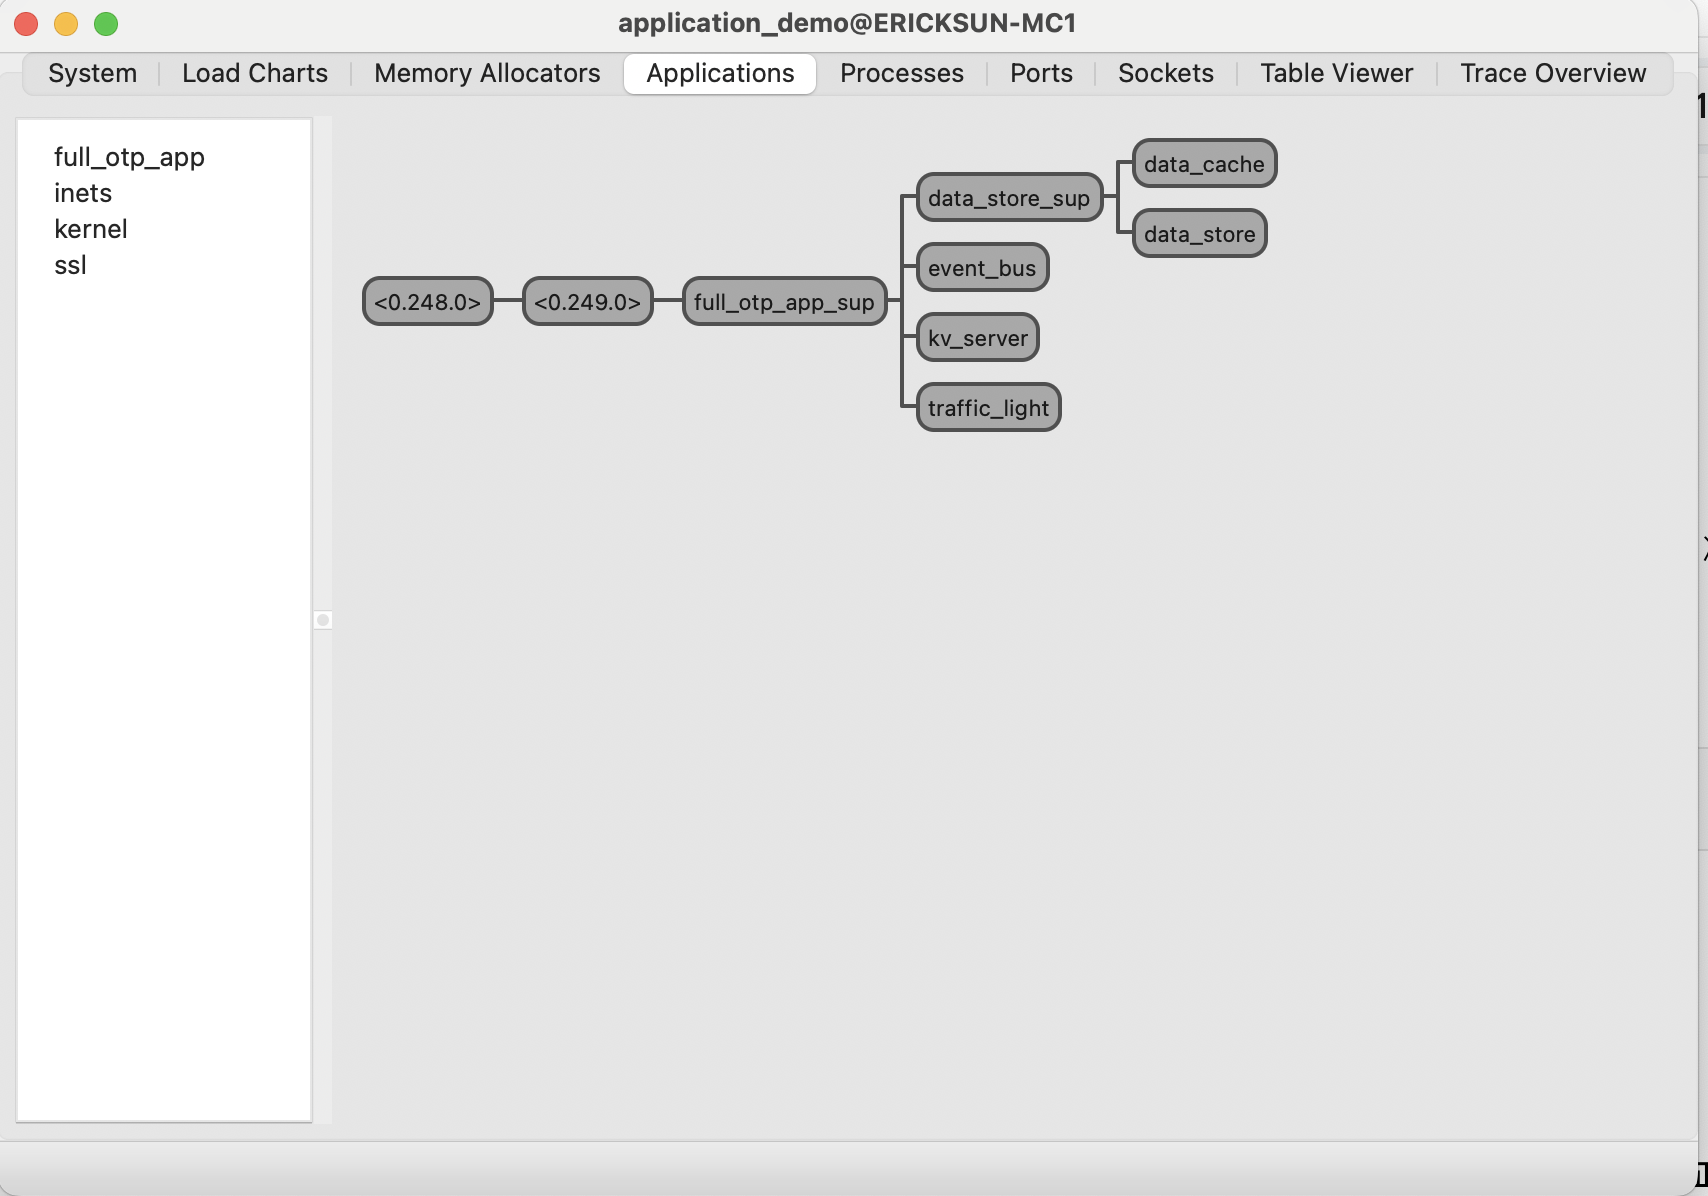
\includegraphics[keepaspectratio]{images/Applications.png}}
\caption{Applications 总览}
\end{figure}

左侧是当前节点启动的 application 列表。常见的系统 application 包括：

\begin{itemize}
\tightlist
\item
  \texttt{kernel}
\item
  \texttt{stdlib}
\item
  \texttt{ssl}
\item
  \texttt{inets}
\item
  自己的业务 application，例如 \texttt{full\_otp\_app}
\end{itemize}

这正好对应 OTP 的第一层结构：application
是一个可启动、可停止、可管理的应用单元。

\begin{center}\rule{0.5\linewidth}{0.5pt}\end{center}

\subsection{7. 观察系统
application}\label{ux89c2ux5bdfux7cfbux7edf-application}

Observer 不只能看自己的应用，也能看 OTP 自带应用。

\subsubsection{7.1 kernel}\label{kernel}

\begin{figure}
\centering
\pandocbounded{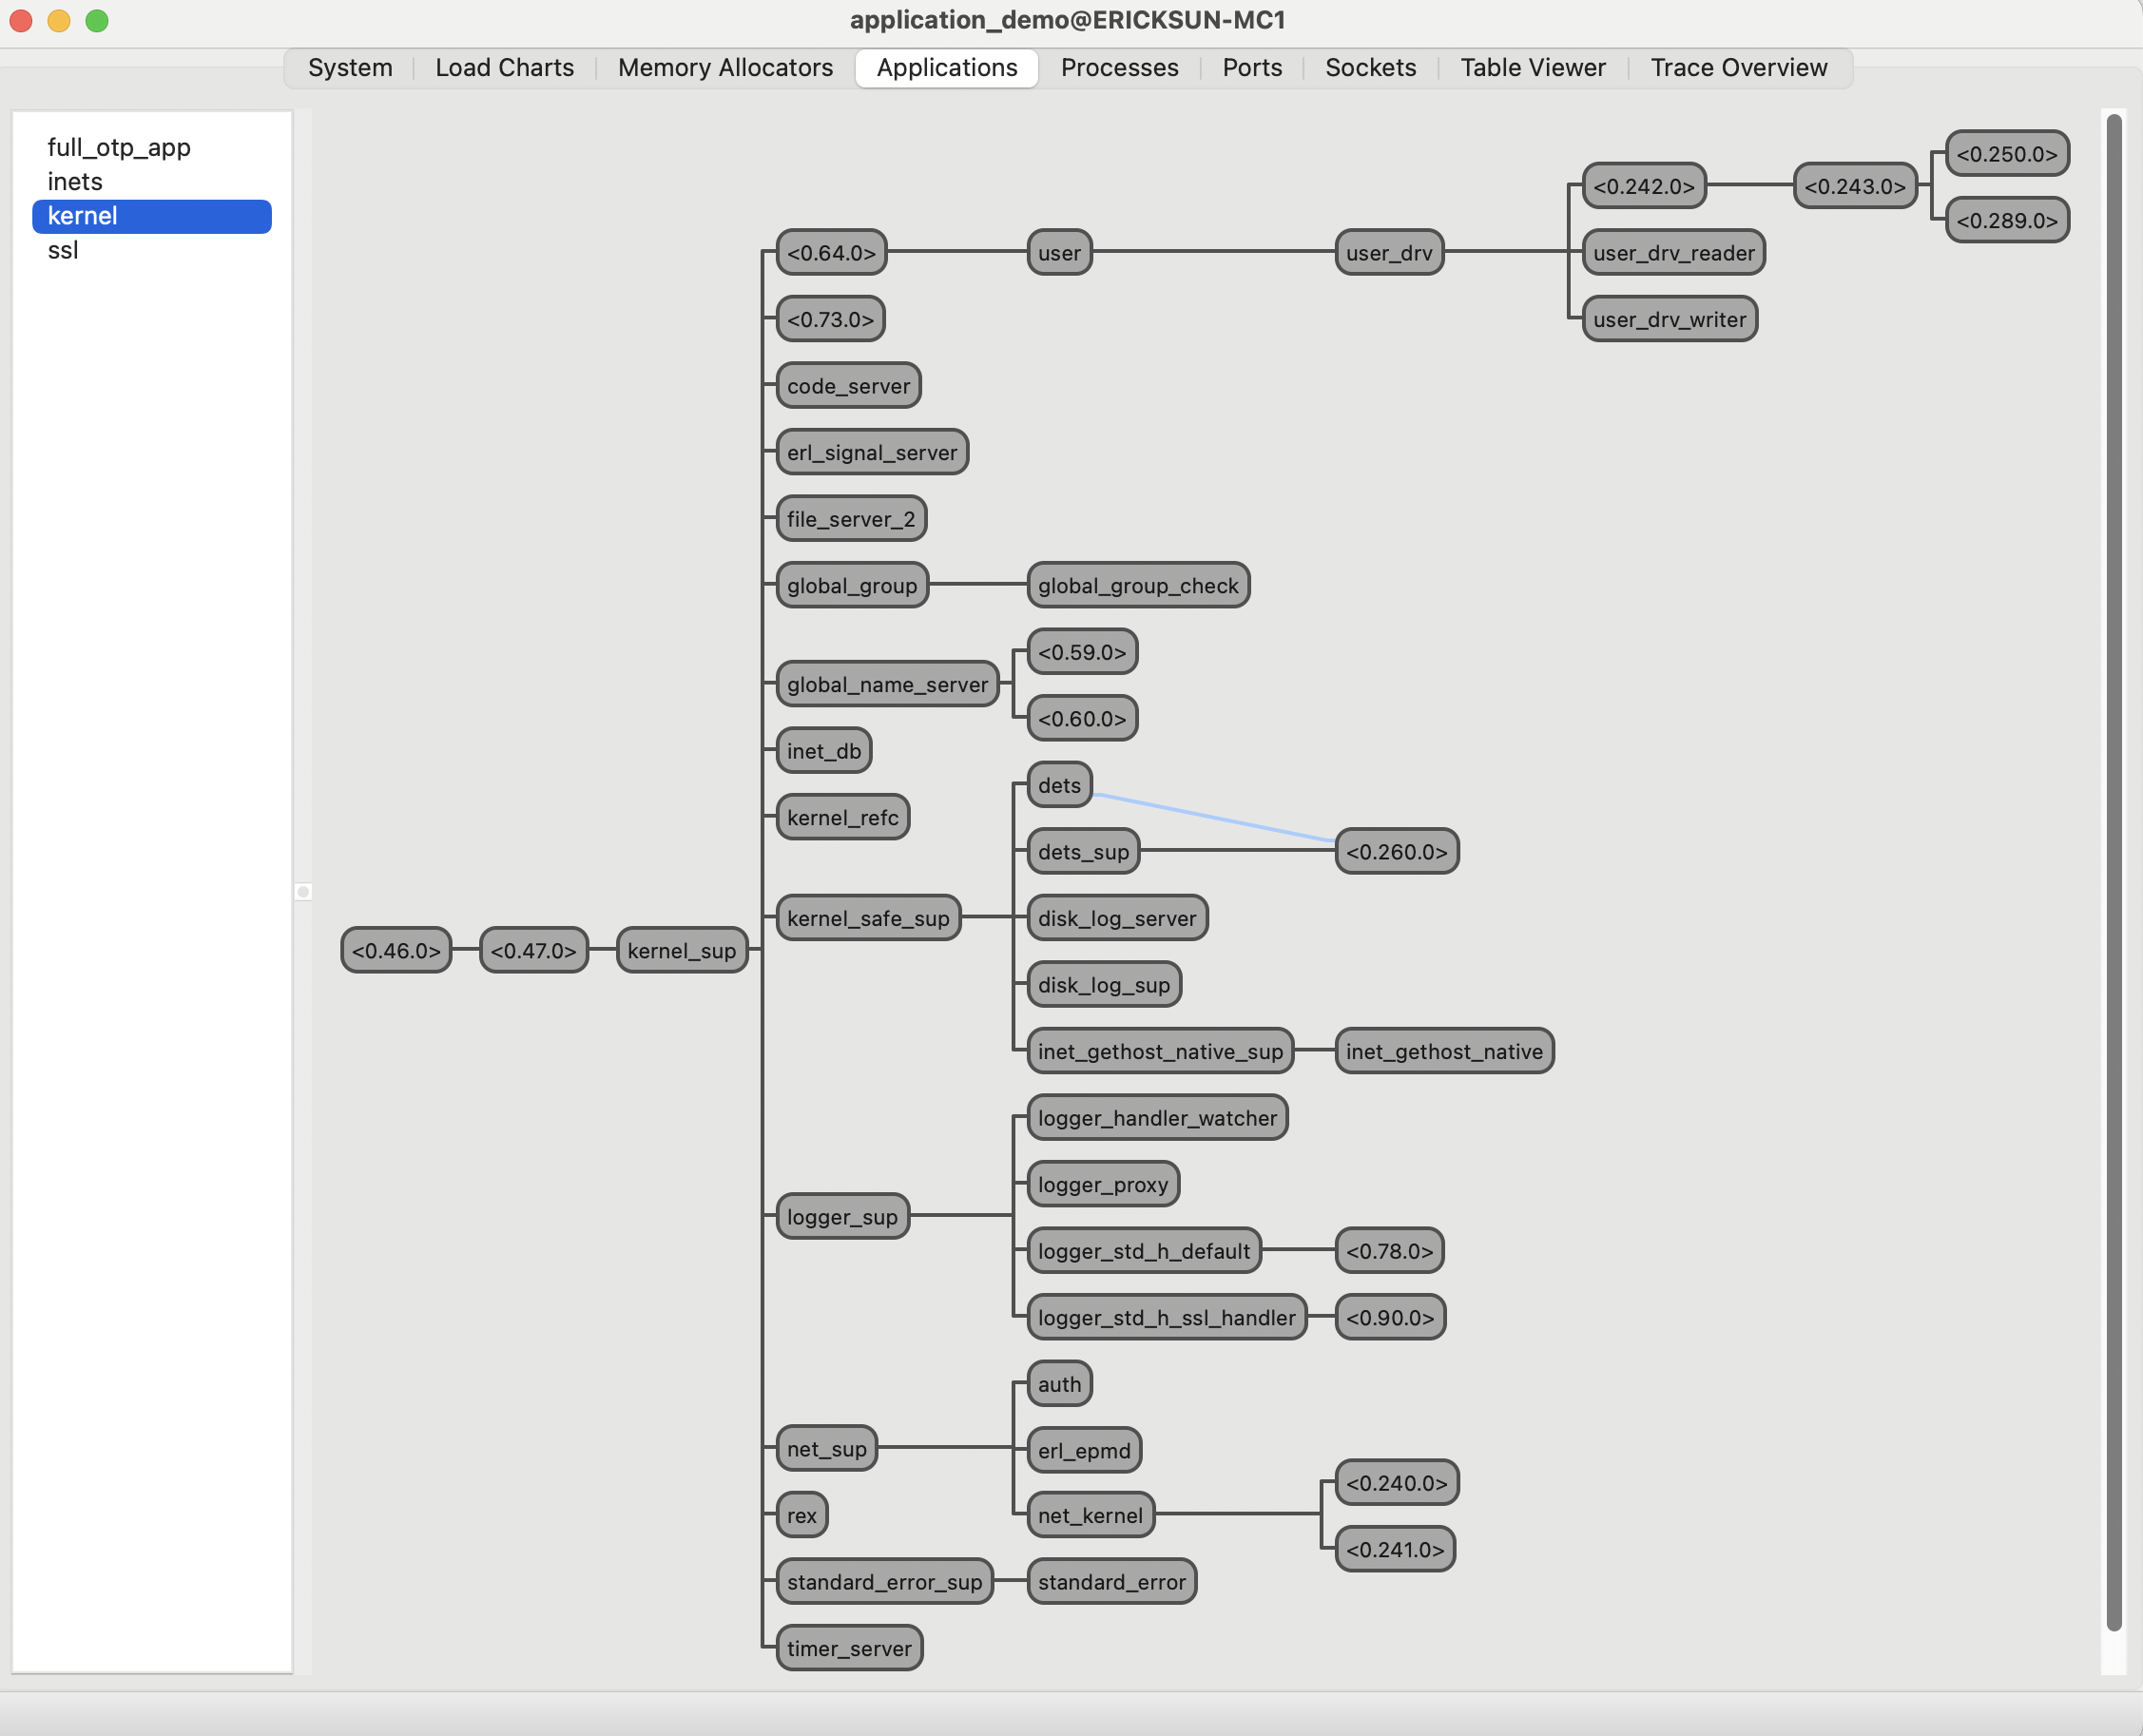
\includegraphics[keepaspectratio]{images/Applications_kernel.png}}
\caption{kernel application}
\end{figure}

\texttt{kernel} 是 Erlang/OTP 最基础的
application，里面包含很多系统级进程。通过这张图可以让学习者理解：OTP
自己也是用 OTP 的方式组织起来的。

\subsubsection{7.2 ssl}\label{ssl}

\begin{figure}
\centering
\pandocbounded{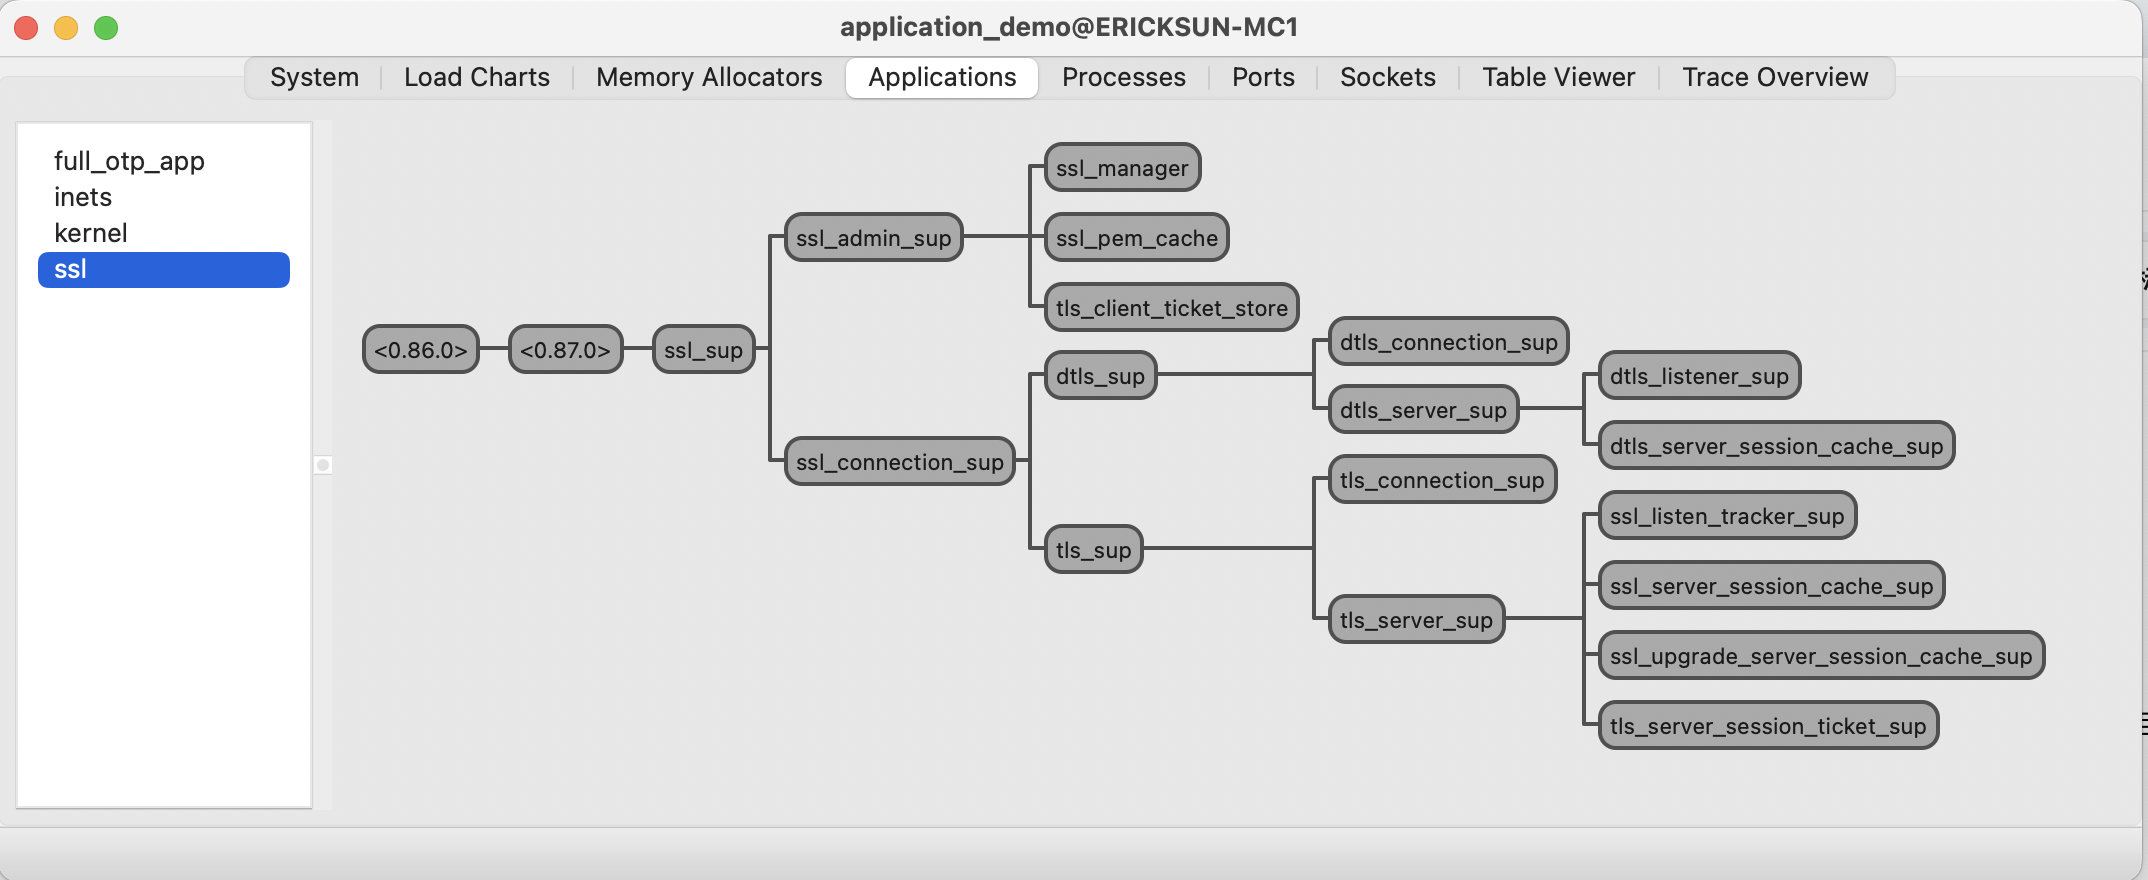
\includegraphics[keepaspectratio]{images/Applications_ssl.png}}
\caption{ssl application}
\end{figure}

\texttt{ssl} application
展示了一个更贴近业务依赖的系统组件。很多网络应用会依赖它。

\subsubsection{7.3 inets}\label{inets}

\begin{figure}
\centering
\pandocbounded{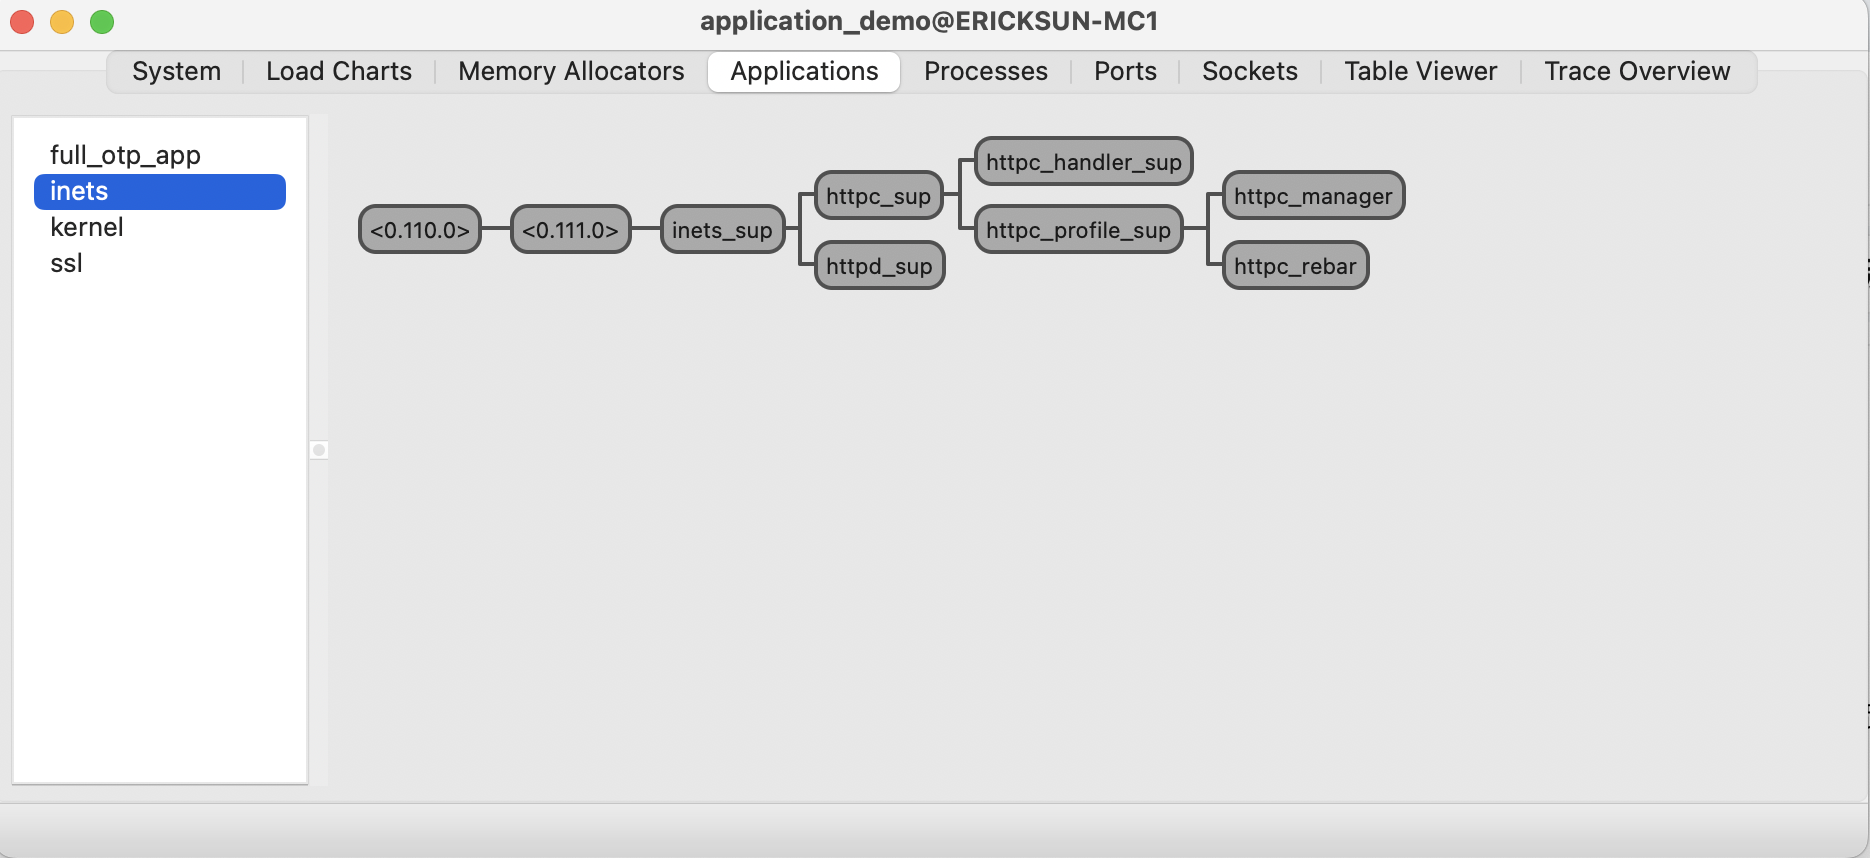
\includegraphics[keepaspectratio]{images/Applications_inets.png}}
\caption{inets application}
\end{figure}

\texttt{inets} 里可以看到一棵 supervision tree。这个例子适合说明：不管是
OTP 内置组件，还是我们自己的应用，Observer 都用同一种方式展示
application 和 supervisor tree。

\begin{center}\rule{0.5\linewidth}{0.5pt}\end{center}

\subsection{8. 观察 full\_otp\_app}\label{ux89c2ux5bdf-full_otp_app}

选中 \texttt{full\_otp\_app} 后，可以看到当前 demo 应用的 supervision
tree。

\begin{figure}
\centering
\pandocbounded{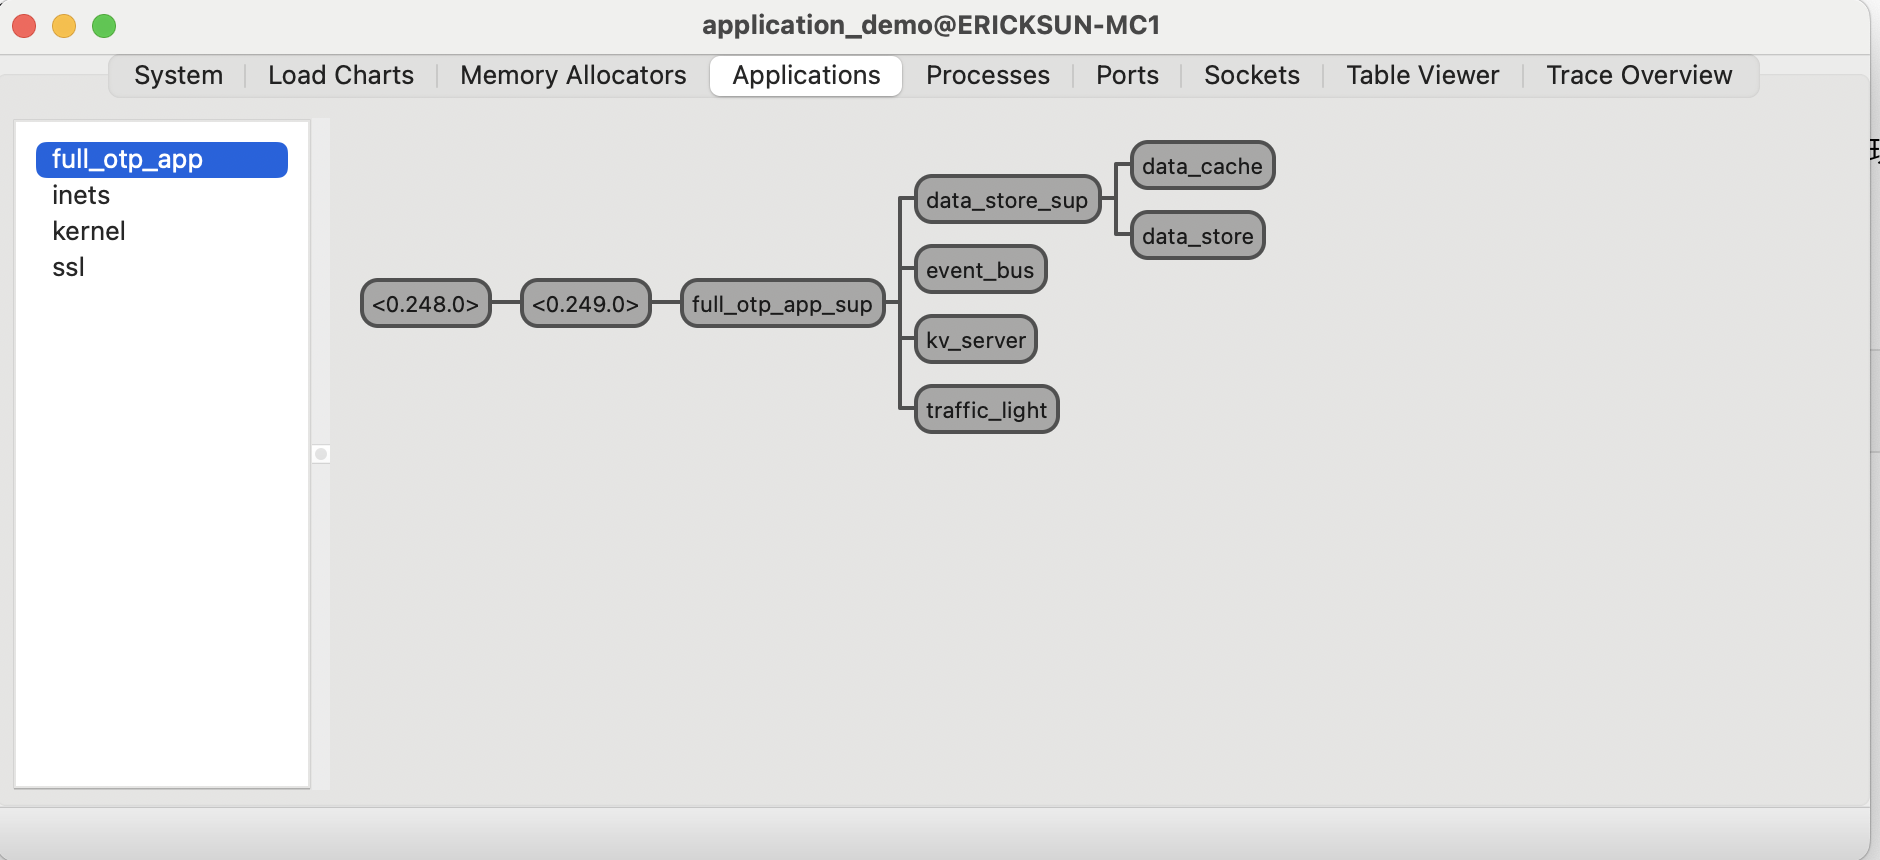
\includegraphics[keepaspectratio]{images/Applications_app.png}}
\caption{full\_otp\_app application}
\end{figure}

这张图是后续讲 application、supervisor、gen\_server、gen\_statem
的总入口。

它对应代码中的 application 配置：

\begin{Shaded}
\begin{Highlighting}[]
\FunctionTok{\{}\CharTok{application}\FunctionTok{,} \CharTok{full\_otp\_app}\FunctionTok{,}
 \FunctionTok{[\{}\CharTok{mod}\FunctionTok{,} \FunctionTok{\{}\CharTok{full\_otp\_app\_app}\FunctionTok{,} \FunctionTok{[]\}\},}
  \FunctionTok{\{}\CharTok{applications}\FunctionTok{,} \FunctionTok{[}\CharTok{kernel}\FunctionTok{,} \CharTok{stdlib}\FunctionTok{,} \CharTok{observer\_cli}\FunctionTok{,} \CharTok{recon}\FunctionTok{]\}]\}.}
\end{Highlighting}
\end{Shaded}

application callback 的职责通常很简单：启动顶层 supervisor。

\begin{Shaded}
\begin{Highlighting}[]
\FunctionTok{start(}\VariableTok{\_StartType}\FunctionTok{,} \VariableTok{\_StartArgs}\FunctionTok{)} \OperatorTok{{-}\textgreater{}}
    \FunctionTok{full\_otp\_app\_sup:start\_link().}
\end{Highlighting}
\end{Shaded}

所以 Observer 里看到的不是``一个 main 函数''，而是一棵运行中的进程树。

\begin{center}\rule{0.5\linewidth}{0.5pt}\end{center}

\subsection{9. Applications 页面里的 supervisor
tree}\label{applications-ux9875ux9762ux91ccux7684-supervisor-tree}

展开 \texttt{full\_otp\_app} 后，可以看到顶层 supervisor 和它的
children。

\begin{figure}
\centering
\pandocbounded{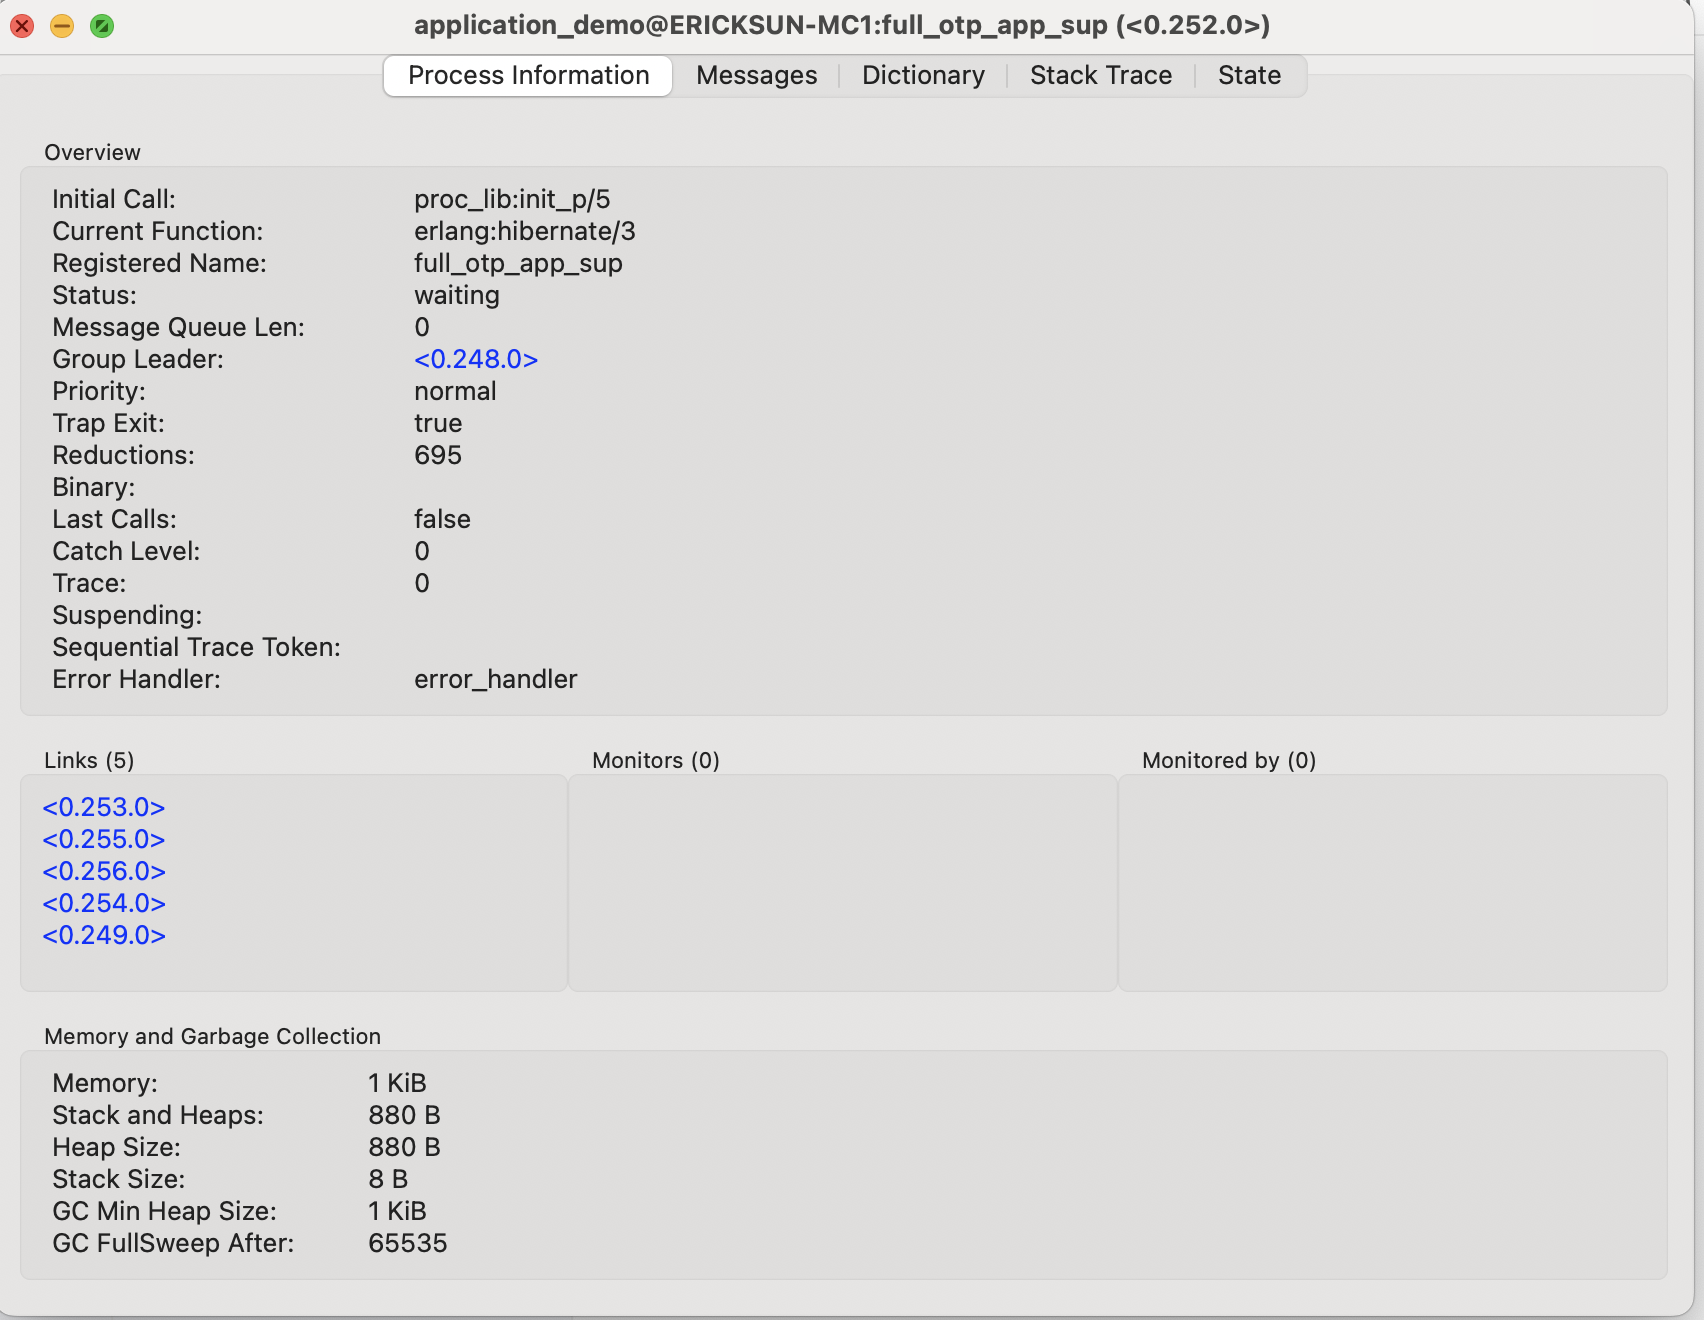
\includegraphics[keepaspectratio]{images/Applications_app_supervisor.png}}
\caption{full\_otp\_app supervisor tree}
\end{figure}

这张图对应 \texttt{full\_otp\_app\_sup:init/1} 里的 child specs：

\begin{Shaded}
\begin{Highlighting}[]
\VariableTok{ChildSpecs} \OperatorTok{=} \FunctionTok{[}
    \FunctionTok{\#\{}\CharTok{id} \OperatorTok{=\textgreater{}} \CharTok{kv\_server}\FunctionTok{,}      \CharTok{start} \OperatorTok{=\textgreater{}} \FunctionTok{\{}\CharTok{kv\_server}\FunctionTok{,} \CharTok{start\_link}\FunctionTok{,} \FunctionTok{[]\},}      \CharTok{type} \OperatorTok{=\textgreater{}} \CharTok{worker}\FunctionTok{\},}
    \FunctionTok{\#\{}\CharTok{id} \OperatorTok{=\textgreater{}} \CharTok{event\_bus}\FunctionTok{,}      \CharTok{start} \OperatorTok{=\textgreater{}} \FunctionTok{\{}\CharTok{event\_bus}\FunctionTok{,} \CharTok{start\_link}\FunctionTok{,} \FunctionTok{[]\},}      \CharTok{type} \OperatorTok{=\textgreater{}} \CharTok{worker}\FunctionTok{\},}
    \FunctionTok{\#\{}\CharTok{id} \OperatorTok{=\textgreater{}} \CharTok{traffic\_light}\FunctionTok{,}  \CharTok{start} \OperatorTok{=\textgreater{}} \FunctionTok{\{}\CharTok{traffic\_light}\FunctionTok{,} \CharTok{start\_link}\FunctionTok{,} \FunctionTok{[]\},}  \CharTok{type} \OperatorTok{=\textgreater{}} \CharTok{worker}\FunctionTok{\},}
    \FunctionTok{\#\{}\CharTok{id} \OperatorTok{=\textgreater{}} \CharTok{data\_store\_sup}\FunctionTok{,} \CharTok{start} \OperatorTok{=\textgreater{}} \FunctionTok{\{}\CharTok{data\_store\_sup}\FunctionTok{,} \CharTok{start\_link}\FunctionTok{,} \FunctionTok{[]\},} \CharTok{type} \OperatorTok{=\textgreater{}} \CharTok{supervisor}\FunctionTok{\}}
\FunctionTok{].}
\end{Highlighting}
\end{Shaded}

重点讲解：

\begin{itemize}
\tightlist
\item
  \texttt{full\_otp\_app\_sup} 是顶层 supervisor。
\item
  \texttt{kv\_server} 是一个 \texttt{gen\_server} worker。
\item
  \texttt{event\_bus} 是一个 \texttt{gen\_event} worker。
\item
  \texttt{traffic\_light} 是一个 \texttt{gen\_statem} worker。
\item
  \texttt{data\_store\_sup} 是子 supervisor。
\item
  \texttt{data\_store\_sup} 下面还有 \texttt{data\_store} 和
  \texttt{data\_cache}。
\end{itemize}

这就是 OTP 的核心直觉：系统不是一堆函数调用，而是一棵由 supervisor
管理的进程树。

另一张 supervisor tree 截图可以用于展示子监督树：

\begin{figure}
\centering
\pandocbounded{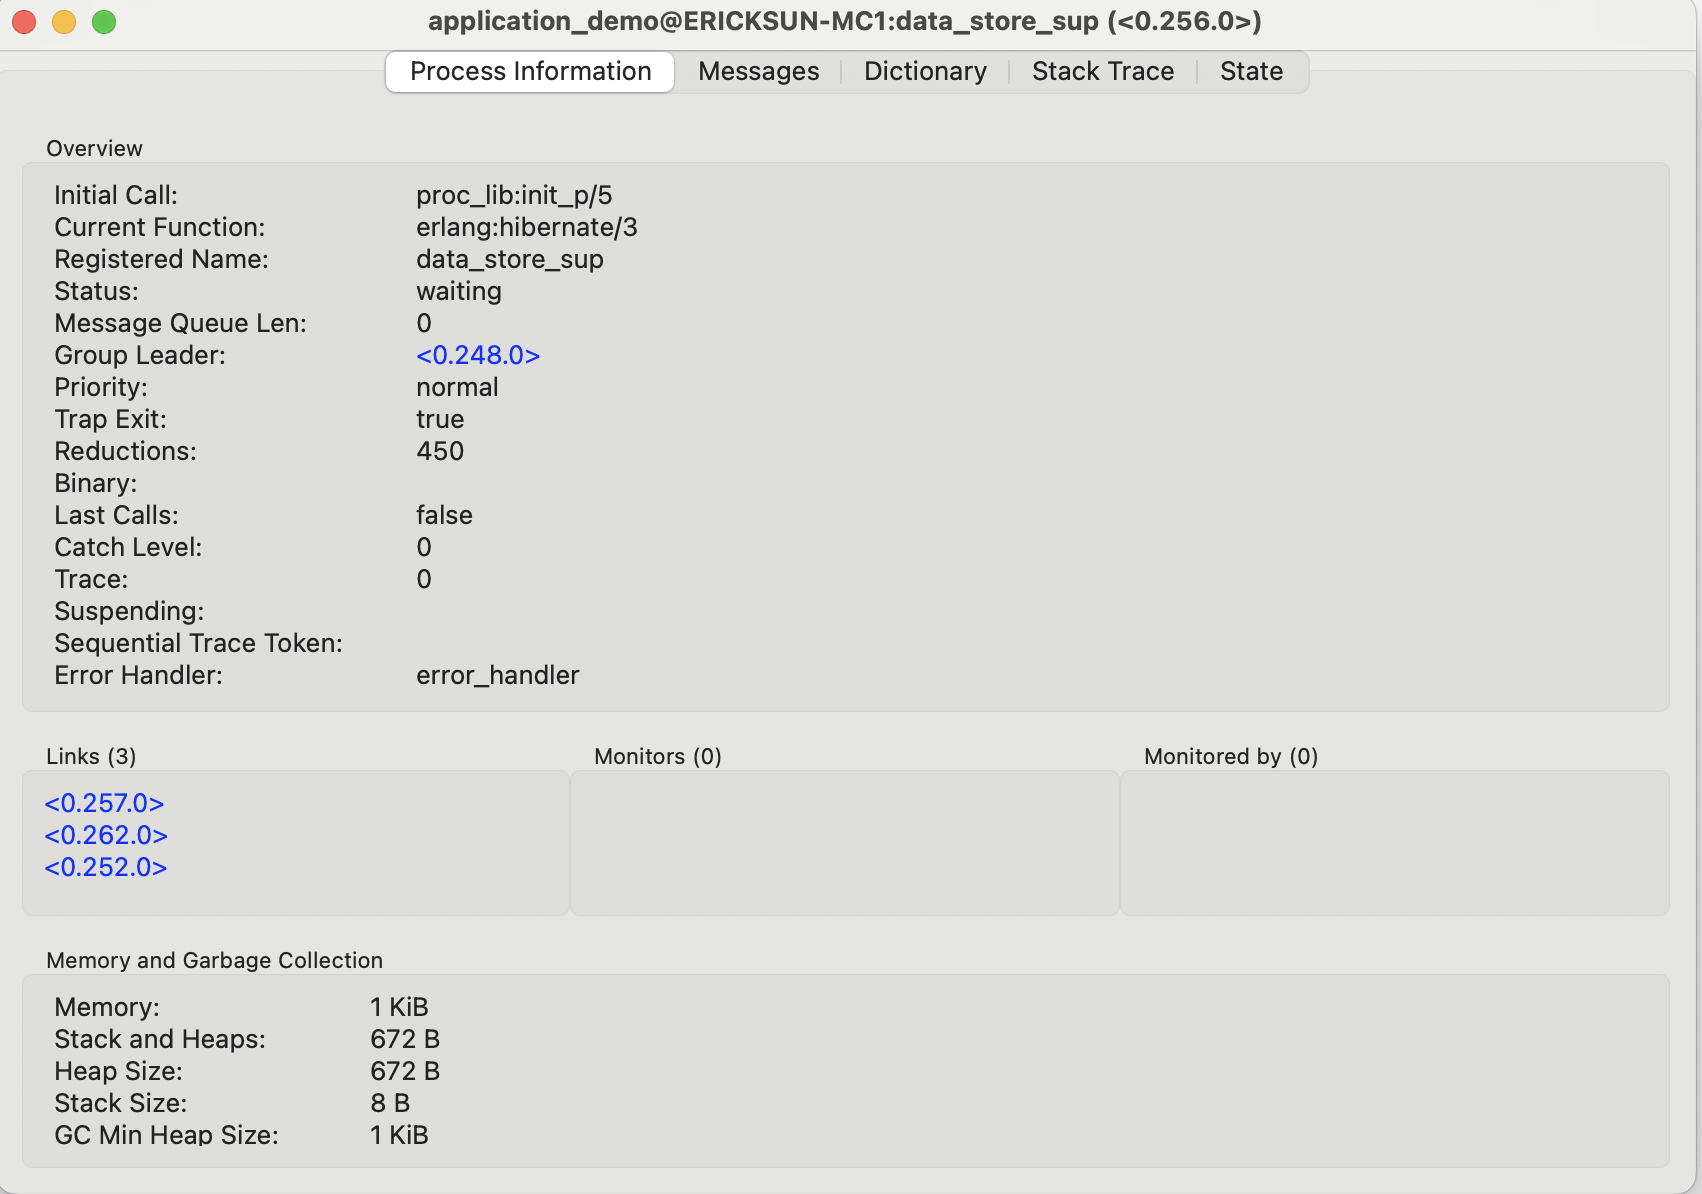
\includegraphics[keepaspectratio]{images/Applications_app_supervisor_second.png}}
\caption{full\_otp\_app 子监督树}
\end{figure}

\begin{center}\rule{0.5\linewidth}{0.5pt}\end{center}

\subsection{10.
Processes：从进程列表看运行时}\label{processesux4eceux8fdbux7a0bux5217ux8868ux770bux8fd0ux884cux65f6}

切换到 \texttt{Processes} 页面，可以看到当前 BEAM 节点中的所有 Erlang
process。

\begin{figure}
\centering
\pandocbounded{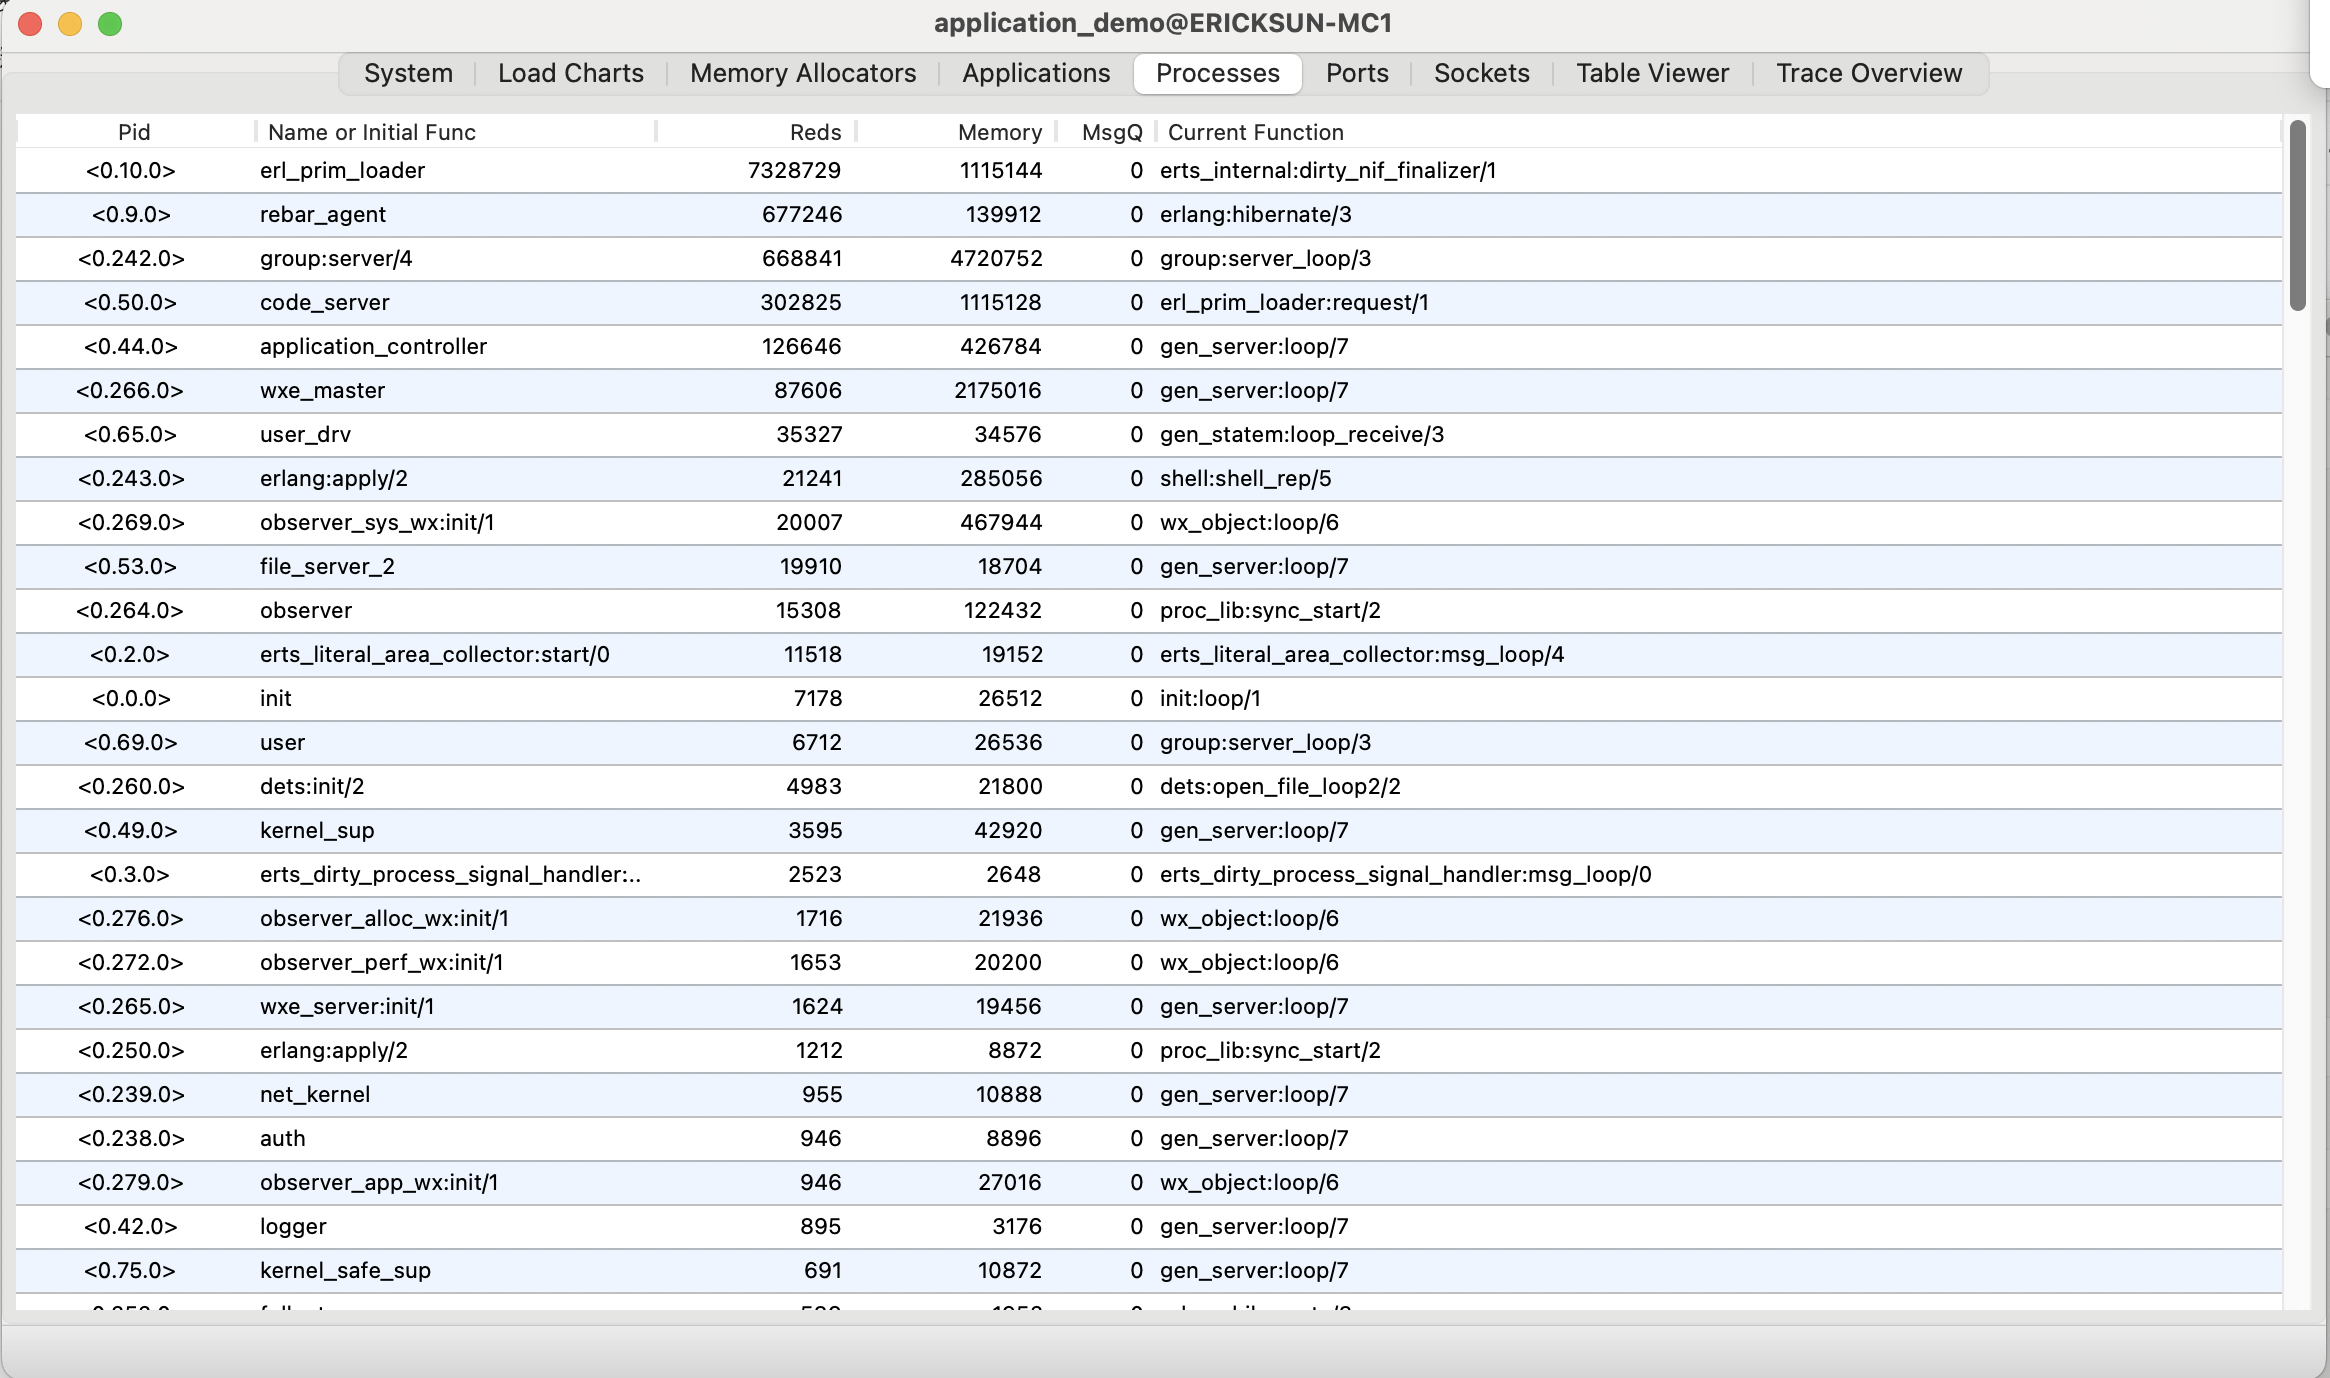
\includegraphics[keepaspectratio]{images/Applications_process_list.png}}
\caption{Processes 列表}
\end{figure}

表格里最重要的列包括：

\begin{longtable}[]{@{}ll@{}}
\toprule\noalign{}
列 & 说明 \\
\midrule\noalign{}
\endhead
\bottomrule\noalign{}
\endlastfoot
Pid & Erlang process id \\
Name or Initial Func & 注册名或初始调用函数 \\
Reds & reductions，近似理解为调度执行量 \\
Memory & 进程占用内存 \\
MsgQ & 消息队列长度 \\
Current Function & 当前正在执行或等待的位置 \\
\end{longtable}

这里建议重点讲 \texttt{MsgQ}。在 Erlang
系统里，进程之间通过消息通信。如果某个进程处理不过来，消息队列长度可能增长。Observer
可以直接看到这一点。

\begin{center}\rule{0.5\linewidth}{0.5pt}\end{center}

\subsection{11. 双击进程：Process
Information}\label{ux53ccux51fbux8fdbux7a0bprocess-information}

在 \texttt{Processes} 页面或 \texttt{Applications}
页面里双击某个进程，可以打开进程详情窗口。

\subsubsection{11.1 supervisor
进程详情}\label{supervisor-ux8fdbux7a0bux8be6ux60c5}

\begin{figure}
\centering
\pandocbounded{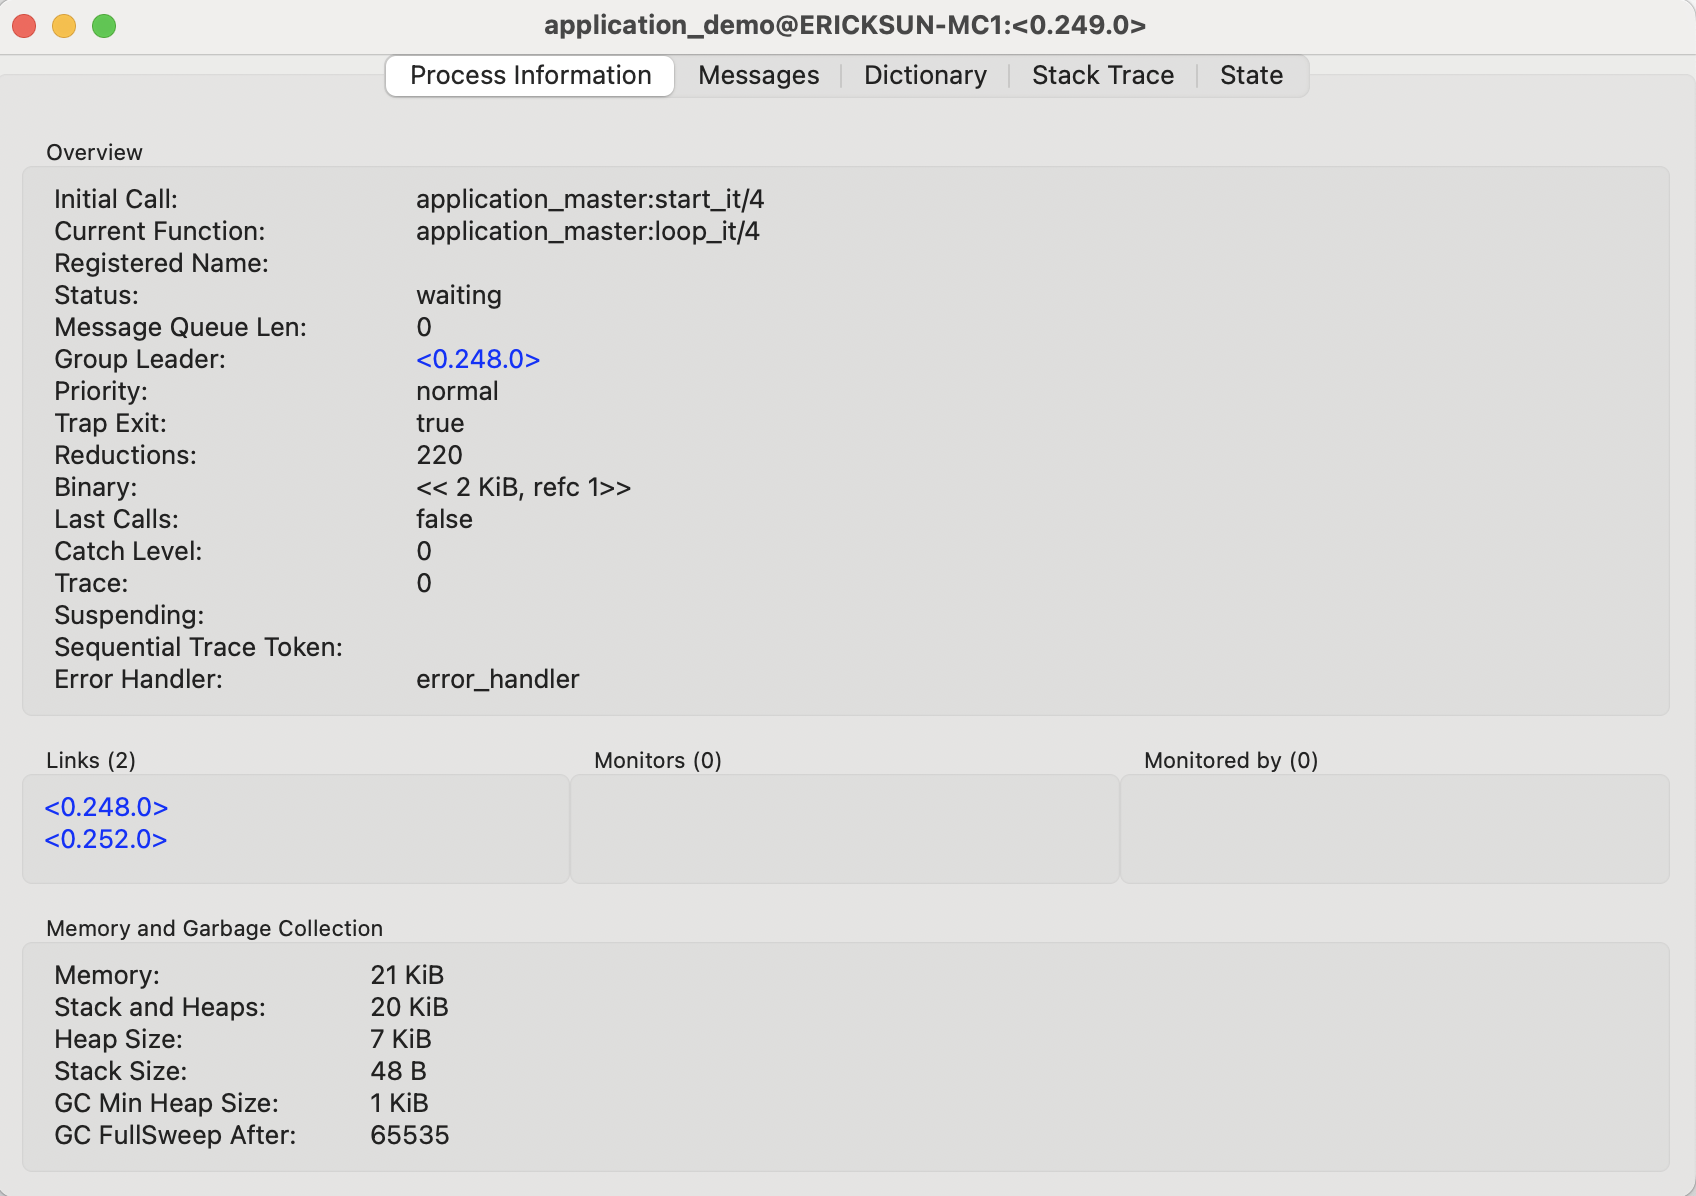
\includegraphics[keepaspectratio]{images/Applications_app_start.png}}
\caption{supervisor Process Information}
\end{figure}

这张图展示的是 \texttt{full\_otp\_app\_sup} 的进程详情。重点观察：

\begin{itemize}
\tightlist
\item
  \texttt{Registered\ Name} 是 \texttt{full\_otp\_app\_sup}。
\item
  \texttt{Current\ Function} 可能是
  \texttt{erlang:hibernate/3}，表示当前空闲等待。
\item
  \texttt{Message\ Queue\ Len} 是消息队列长度。
\item
  \texttt{Links} 显示它链接到哪些子进程或相关进程。
\item
  \texttt{Trap\ Exit} 对 supervisor
  很重要，因为它需要接收子进程退出信号。
\end{itemize}

这可以帮助解释：supervisor 不是抽象配置，它本身就是一个真实运行的 Erlang
process。

\subsubsection{11.2 gen\_server
进程详情：kv\_server}\label{gen_server-ux8fdbux7a0bux8be6ux60c5kv_server}

\begin{figure}
\centering
\pandocbounded{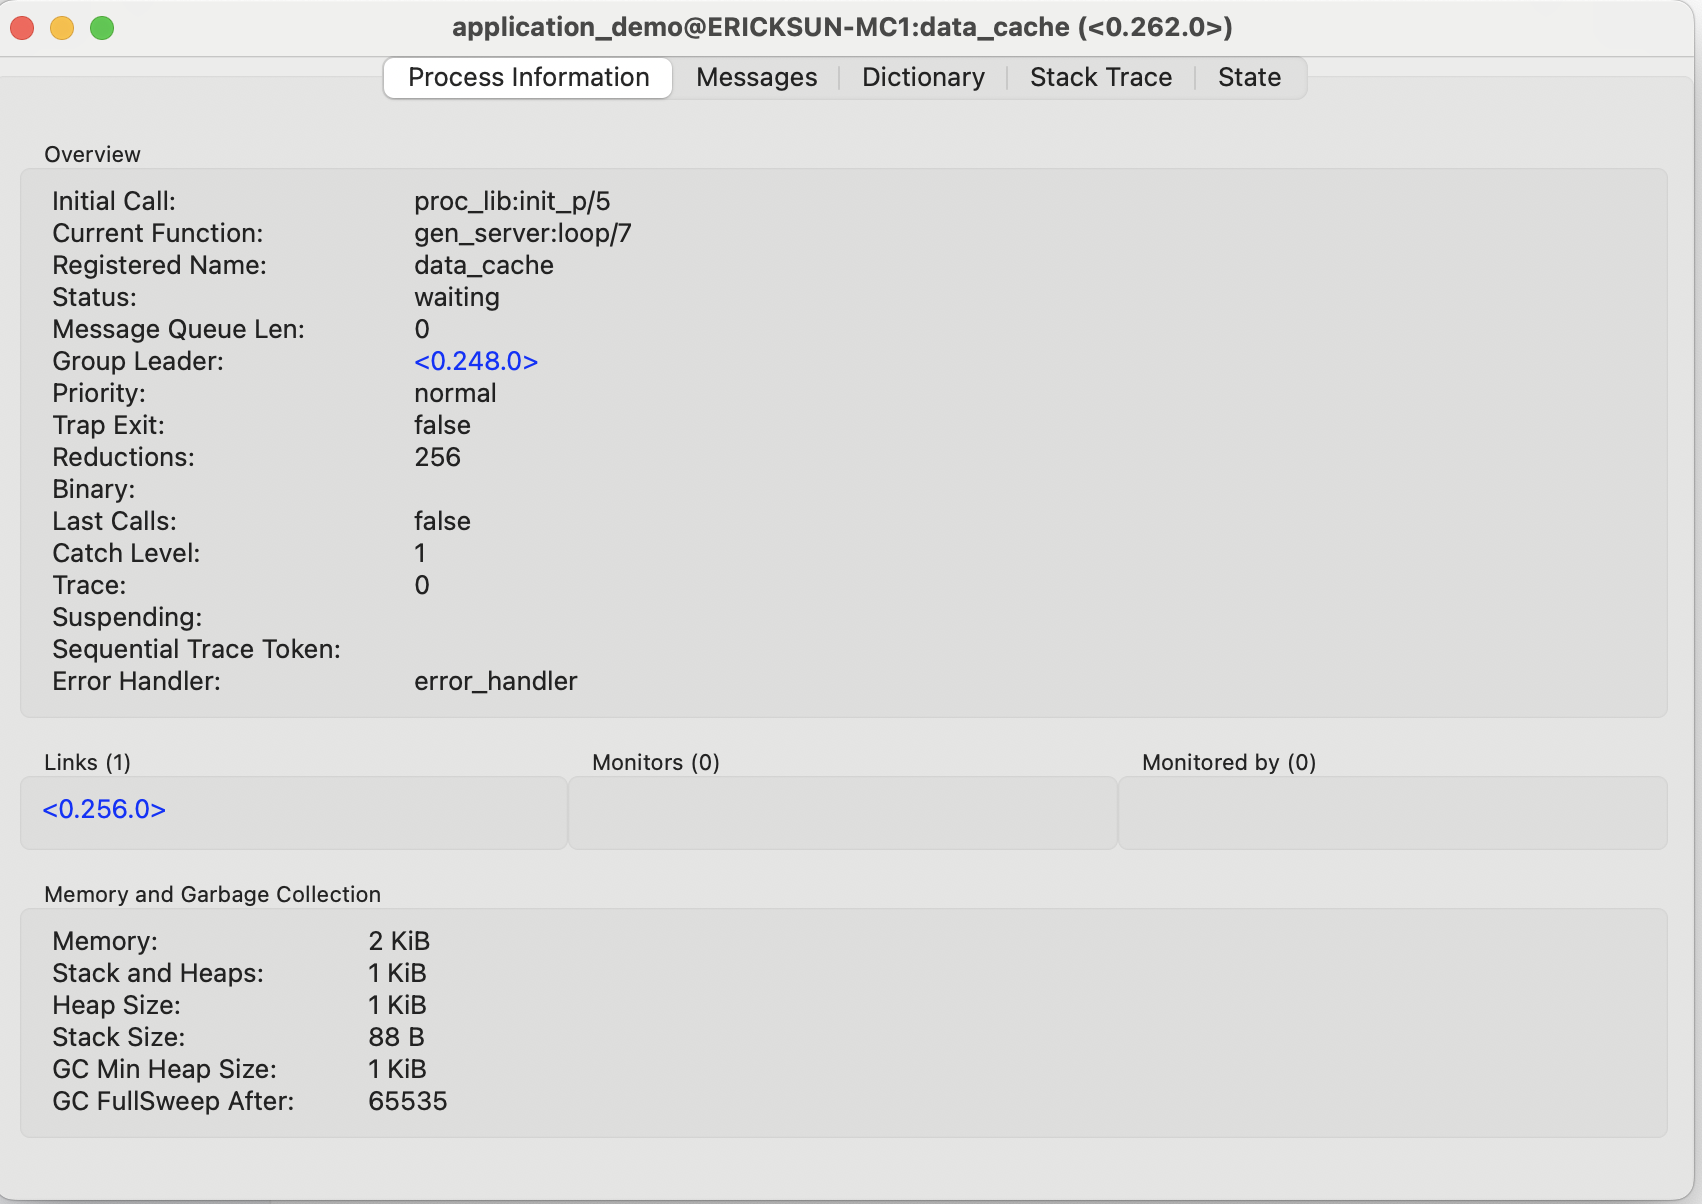
\includegraphics[keepaspectratio]{images/Applications_app_gen_server_process.png}}
\caption{kv\_server Process Information}
\end{figure}

\texttt{kv\_server} 是 demo 中的 key-value store，对应源码
\texttt{kv\_server.erl}。

它的 API 包括：

\begin{Shaded}
\begin{Highlighting}[]
\FunctionTok{kv\_server:put(}\CharTok{name}\FunctionTok{,} \StringTok{"Erlang"}\FunctionTok{).}
\FunctionTok{kv\_server:get(}\CharTok{name}\FunctionTok{).}
\FunctionTok{kv\_server:delete(}\CharTok{name}\FunctionTok{).}
\FunctionTok{kv\_server:all().}
\FunctionTok{kv\_server:clear().}
\end{Highlighting}
\end{Shaded}

在进程详情里可以重点观察：

\begin{itemize}
\tightlist
\item
  \texttt{Registered\ Name} 是 \texttt{kv\_server}。
\item
  \texttt{Current\ Function} 通常是 \texttt{gen\_server:loop/7}。
\item
  \texttt{Message\ Queue\ Len} 可以观察是否堆积消息。
\item
  \texttt{Memory} 和 \texttt{Reductions} 可以观察进程资源消耗。
\end{itemize}

这时再回到代码讲
\texttt{handle\_call/3}、\texttt{handle\_cast/2}、\texttt{handle\_info/2}，学习者会更容易理解：这些
callback 是运行中进程处理消息的入口。

\begin{center}\rule{0.5\linewidth}{0.5pt}\end{center}

\subsection{12. State：查看 OTP behaviour
状态}\label{stateux67e5ux770b-otp-behaviour-ux72b6ux6001}

Process Information 窗口上方有多个 tab：

\begin{Shaded}
\begin{Highlighting}[]
\NormalTok{Process Information | Messages | Dictionary | Stack Trace | State}
\end{Highlighting}
\end{Shaded}

其中 \texttt{State} 对学习 OTP 特别有价值，因为它能显示
\texttt{gen\_server} 或 \texttt{gen\_statem} 的内部状态。

\subsubsection{12.1 kv\_server 的 State}\label{kv_server-ux7684-state}

\begin{figure}
\centering
\pandocbounded{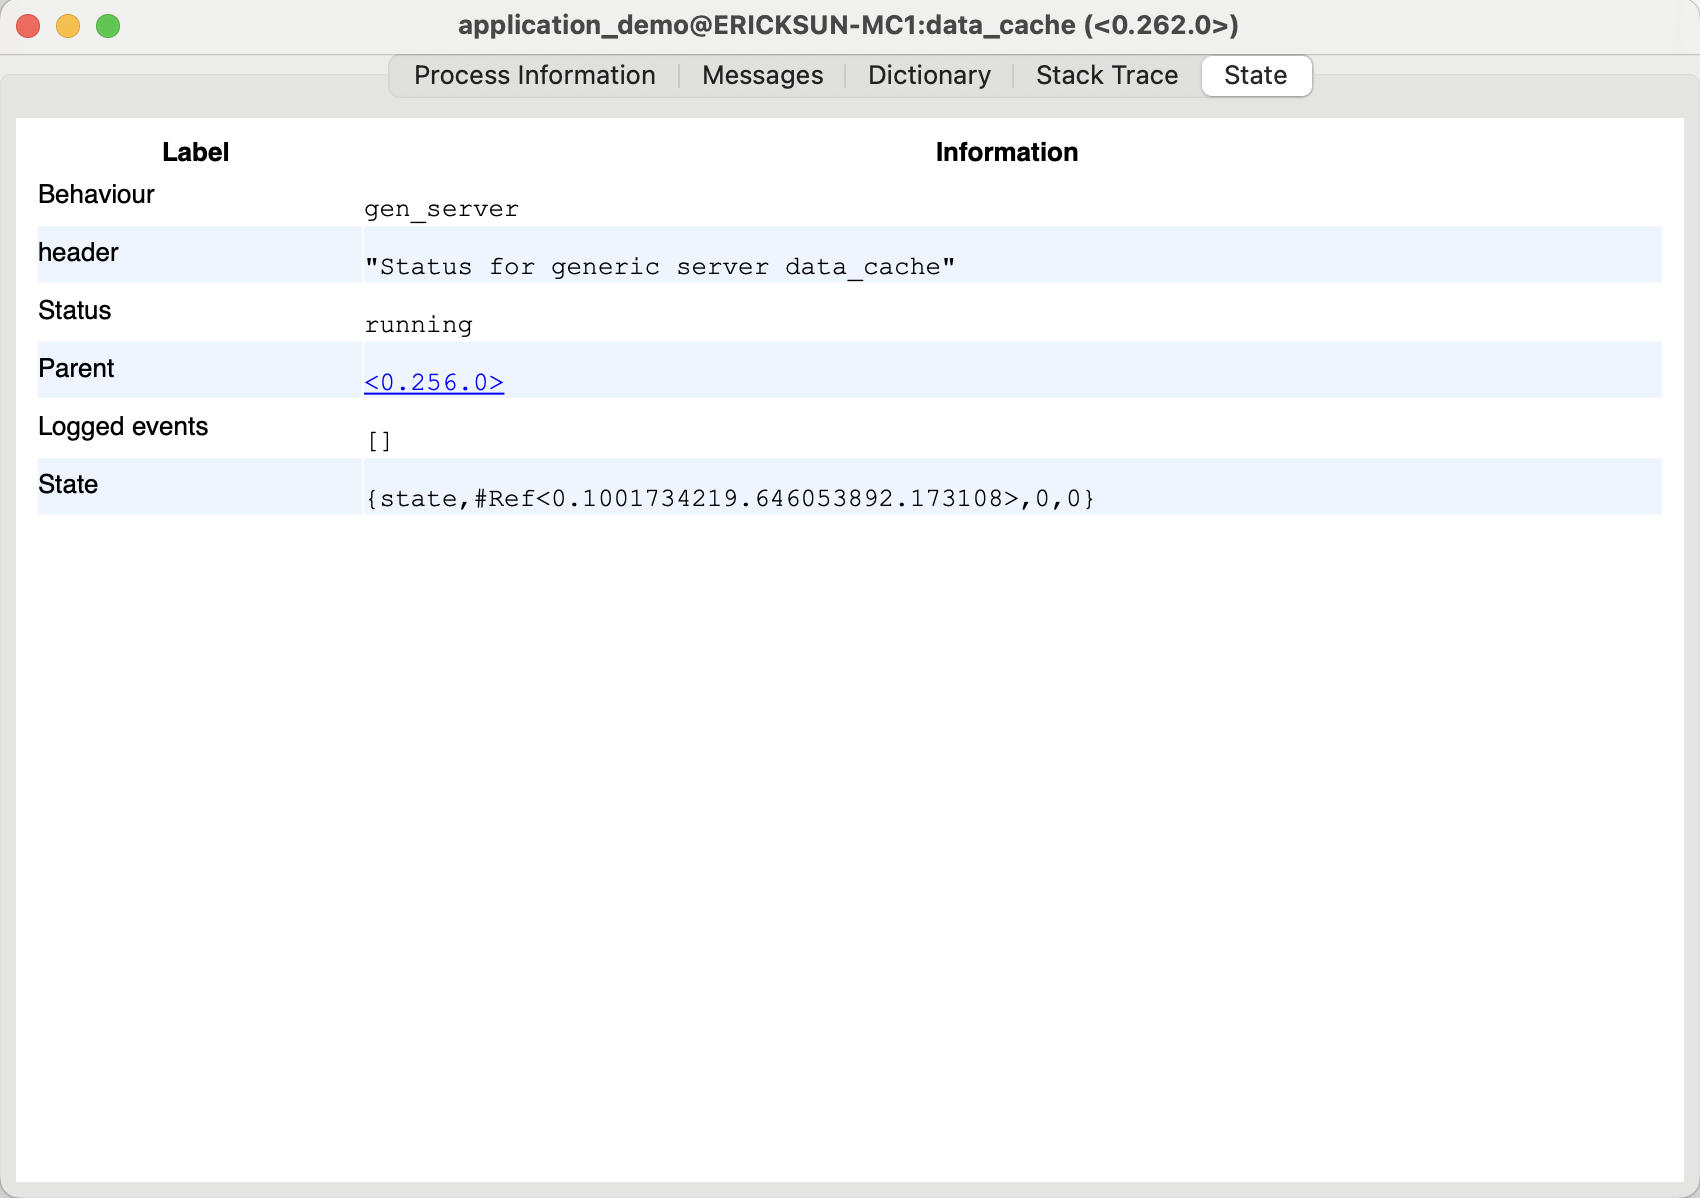
\includegraphics[keepaspectratio]{images/Applications_app_gen_server_state.png}}
\caption{kv\_server State}
\end{figure}

\texttt{kv\_server} 的状态是一个 record：

\begin{Shaded}
\begin{Highlighting}[]
\OperatorTok{{-}}\FunctionTok{record(}\CharTok{state}\FunctionTok{,} \FunctionTok{\{}
    \CharTok{store} \OperatorTok{=} \FunctionTok{\#\{\}} \FunctionTok{::} \FunctionTok{map(),}
    \CharTok{ops\_count} \OperatorTok{=} \DecValTok{0} \FunctionTok{::} \FunctionTok{non\_neg\_integer()}
\FunctionTok{\}).}
\end{Highlighting}
\end{Shaded}

当执行：

\begin{Shaded}
\begin{Highlighting}[]
\FunctionTok{kv\_server:put(}\CharTok{language}\FunctionTok{,} \StringTok{"Erlang"}\FunctionTok{).}
\FunctionTok{kv\_server:put(}\CharTok{version}\FunctionTok{,} \StringTok{"OTP 27"}\FunctionTok{).}
\end{Highlighting}
\end{Shaded}

再查看 \texttt{State} 页面，就可以看到内部 map 和操作计数的变化。

这能非常直观地说明：\texttt{gen\_server} 的 State
不是全局变量，也不是类成员变量，而是某个 Erlang process 私有持有的数据。

\subsubsection{12.2 data\_store / data\_cache
进程详情}\label{data_store-data_cache-ux8fdbux7a0bux8be6ux60c5}

\begin{figure}
\centering
\pandocbounded{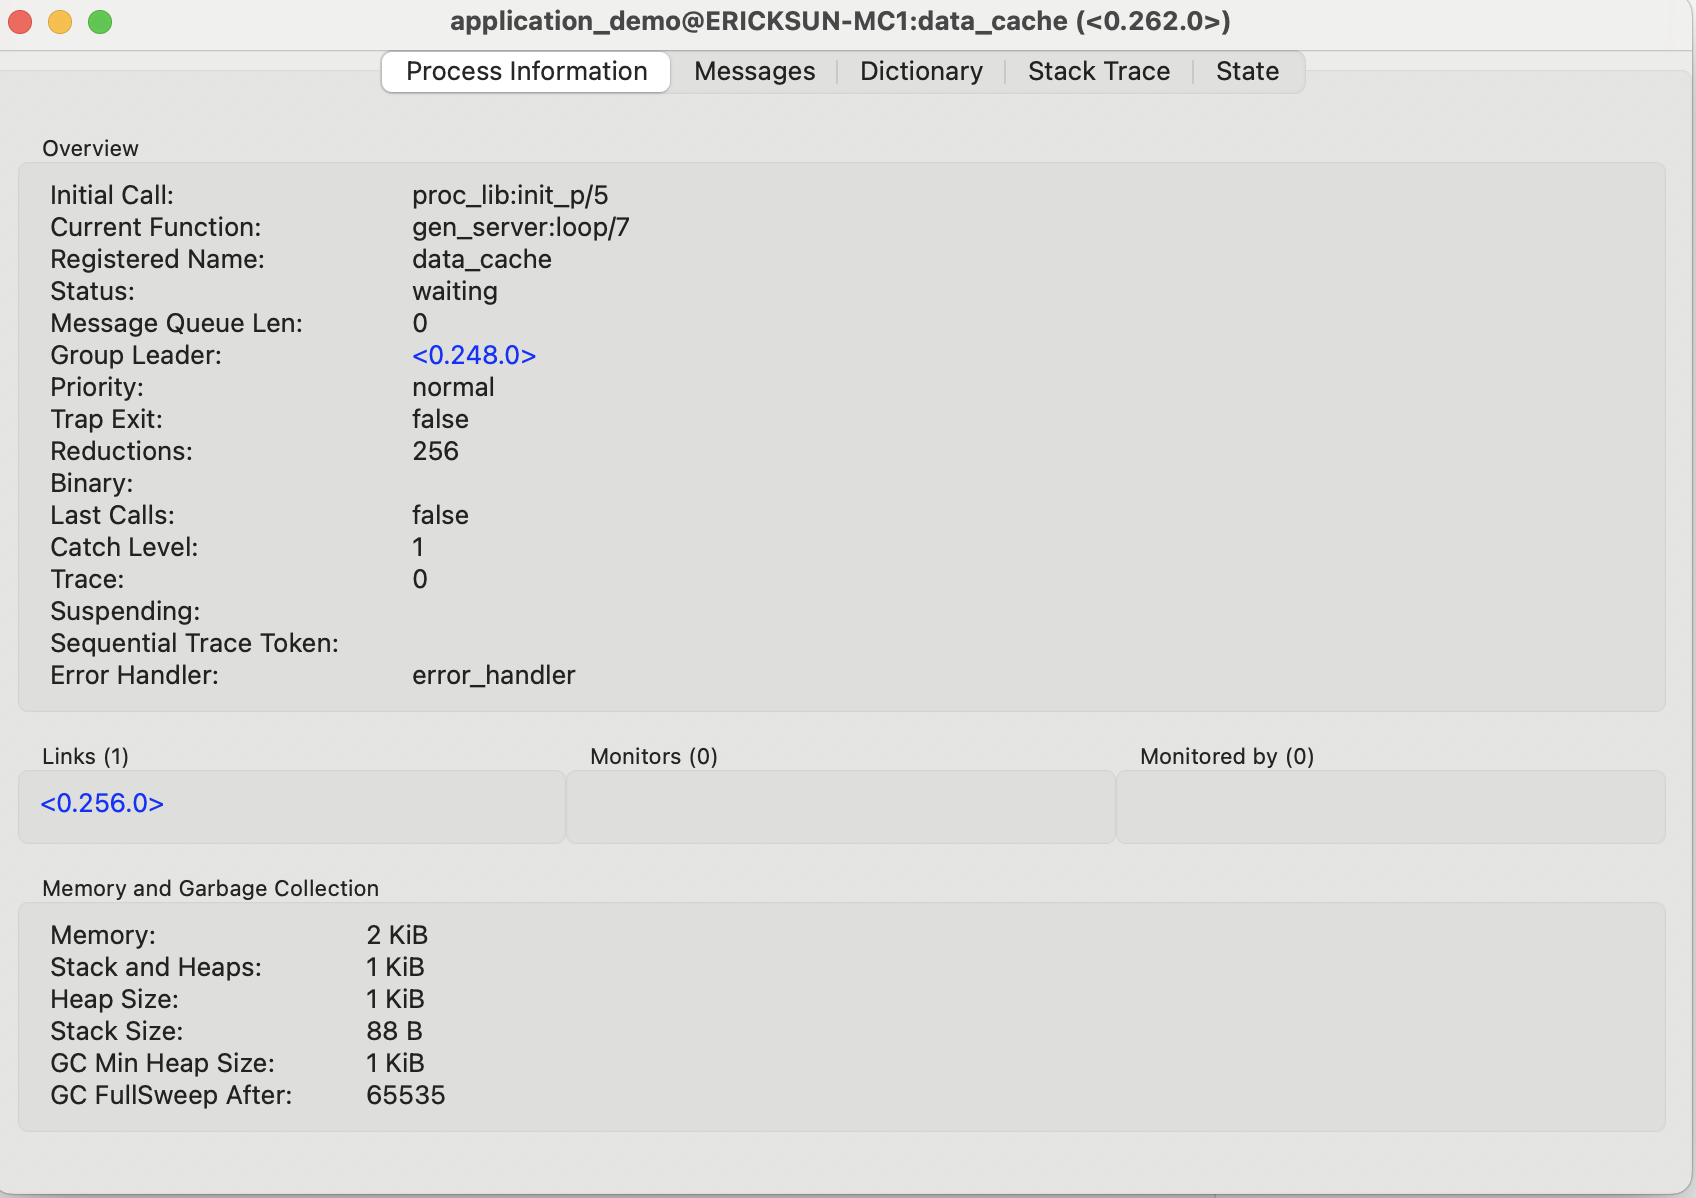
\includegraphics[keepaspectratio]{images/Applications_app_gen_server_process_data_store.png}}
\caption{data\_store Process Information}
\end{figure}

\texttt{data\_store} 是基于 DETS 的持久化进程，\texttt{data\_cache} 是
ETS 缓存进程。它们由 \texttt{data\_store\_sup} 这个子 supervisor 管理。

\texttt{data\_cache} 的状态截图：

\begin{figure}
\centering
\pandocbounded{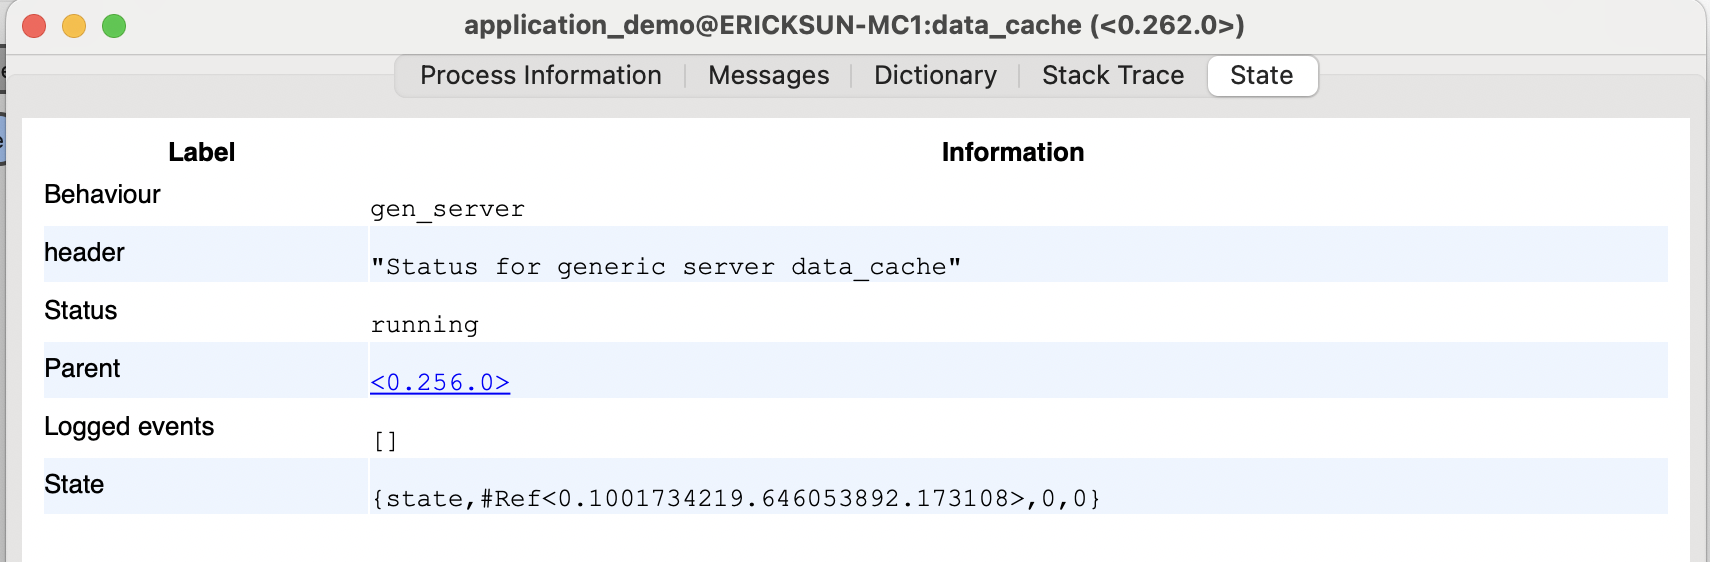
\includegraphics[keepaspectratio]{images/Applications_app_gen_server_process_data_store_state.png}}
\caption{data\_cache State}
\end{figure}

这个例子适合说明两点：

\begin{enumerate}
\def\labelenumi{\arabic{enumi}.}
\tightlist
\item
  OTP 系统中可以有 supervisor under supervisor。
\item
  每个 worker 都可以单独观察它的进程信息和状态。
\end{enumerate}

\begin{center}\rule{0.5\linewidth}{0.5pt}\end{center}

\subsection{13.
gen\_statem：观察状态机进程}\label{gen_statemux89c2ux5bdfux72b6ux6001ux673aux8fdbux7a0b}

\texttt{traffic\_light} 是一个
\texttt{gen\_statem}，用来模拟红绿灯状态机。

状态转换如下：

\begin{Shaded}
\begin{Highlighting}[]
\NormalTok{red {-}\textgreater{} green {-}\textgreater{} yellow {-}\textgreater{} red}
\end{Highlighting}
\end{Shaded}

也支持外部事件：

\begin{Shaded}
\begin{Highlighting}[]
\FunctionTok{traffic\_light:current\_state().}
\FunctionTok{traffic\_light:next().}
\FunctionTok{traffic\_light:emergency().}
\FunctionTok{traffic\_light:resume().}
\end{Highlighting}
\end{Shaded}

\subsubsection{13.1 traffic\_light
进程详情}\label{traffic_light-ux8fdbux7a0bux8be6ux60c5}

\begin{figure}
\centering
\pandocbounded{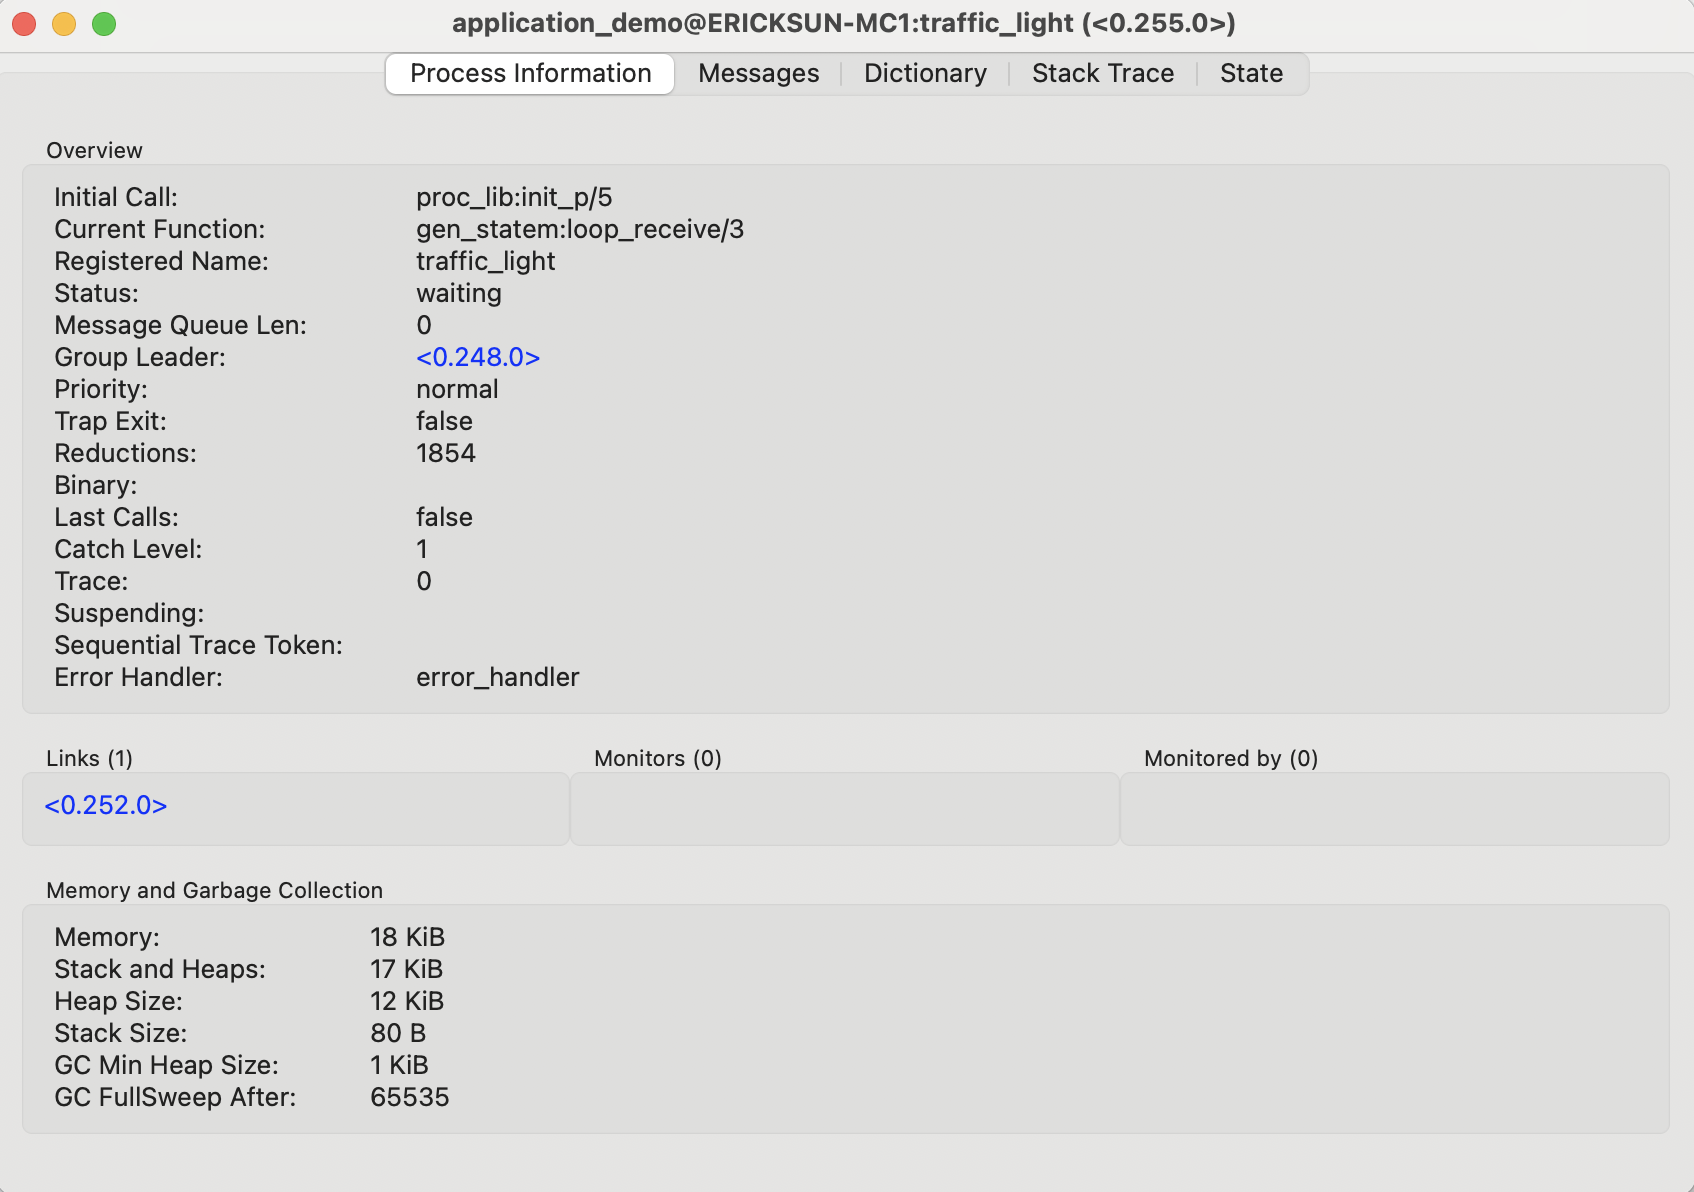
\includegraphics[keepaspectratio]{images/Applications_app_traffic_light_process.png}}
\caption{traffic\_light Process Information}
\end{figure}

可以看到它也是一个普通 Erlang process，只是 current function 和 State
展示会体现 \texttt{gen\_statem} 的运行模型。

\subsubsection{13.2 traffic\_light 的
State}\label{traffic_light-ux7684-state}

\begin{figure}
\centering
\pandocbounded{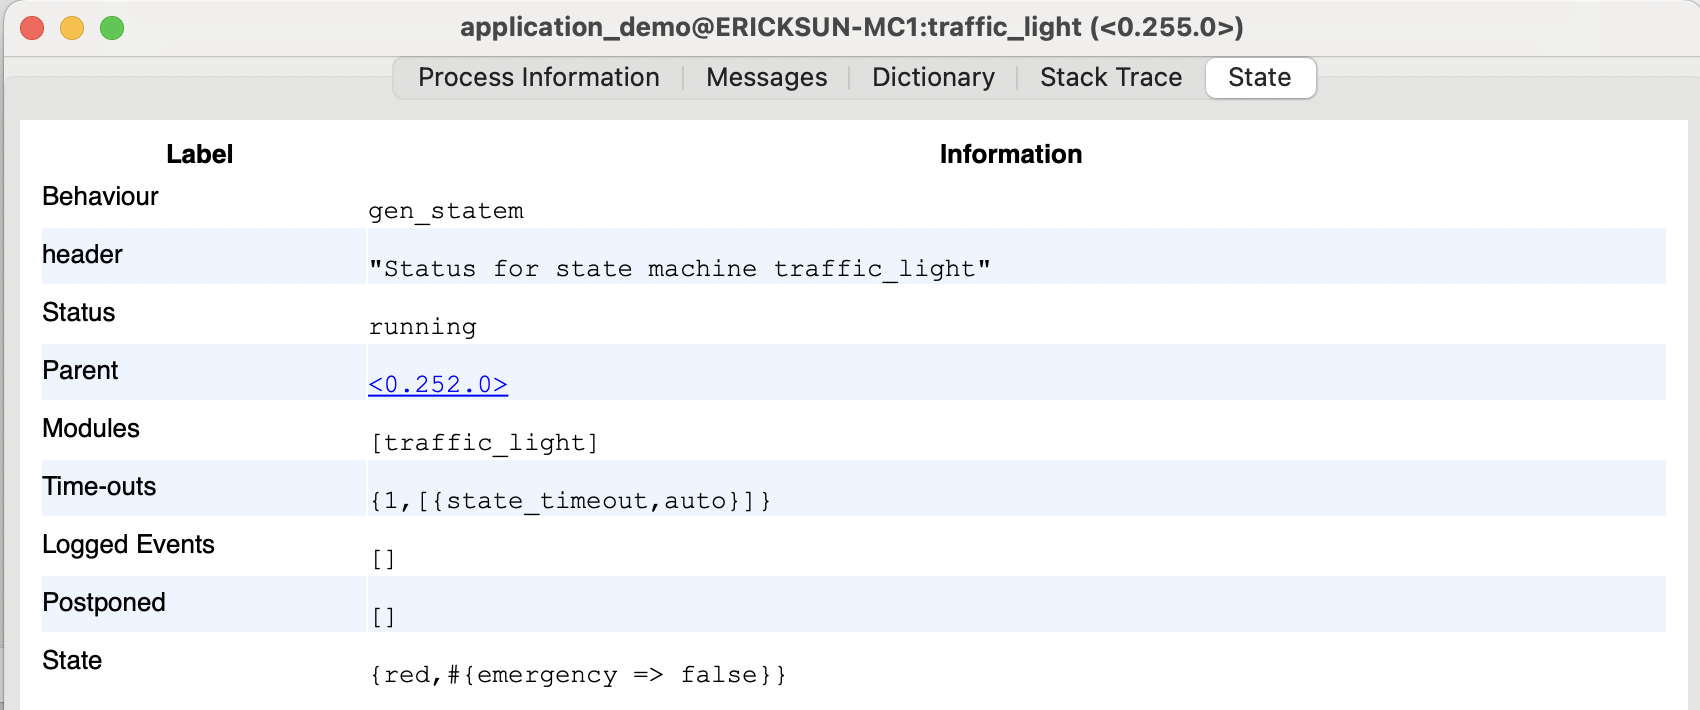
\includegraphics[keepaspectratio]{images/Applications_app_traffic_light_state.png}}
\caption{traffic\_light State}
\end{figure}

\texttt{State} 页面里能看到：

\begin{itemize}
\tightlist
\item
  Behaviour 是 \texttt{gen\_statem}。
\item
  当前状态机状态，例如 \texttt{red}。
\item
  状态数据，例如 \texttt{\#\{emergency\ =\textgreater{}\ false\}}。
\item
  timeout 信息，例如 \texttt{\{state\_timeout,\ auto\}}。
\end{itemize}

这张图非常适合讲 \texttt{gen\_server} 和 \texttt{gen\_statem} 的区别：

\begin{itemize}
\tightlist
\item
  \texttt{gen\_server} 更像``长期运行的状态服务''。
\item
  \texttt{gen\_statem} 更像``显式状态机''。
\item
  Observer 能直接看到当前状态机状态和数据。
\end{itemize}

\begin{center}\rule{0.5\linewidth}{0.5pt}\end{center}

\subsection{14. Messages / Dictionary / Stack
Trace：继续深入进程内部}\label{messages-dictionary-stack-traceux7ee7ux7eedux6df1ux5165ux8fdbux7a0bux5185ux90e8}

进程详情窗口里除了 \texttt{State}，还有几个非常适合调试的 tab：

\begin{longtable}[]{@{}
  >{\raggedright\arraybackslash}p{(\linewidth - 4\tabcolsep) * \real{0.2000}}
  >{\raggedright\arraybackslash}p{(\linewidth - 4\tabcolsep) * \real{0.2400}}
  >{\raggedright\arraybackslash}p{(\linewidth - 4\tabcolsep) * \real{0.5600}}@{}}
\toprule\noalign{}
\begin{minipage}[b]{\linewidth}\raggedright
Tab
\end{minipage} & \begin{minipage}[b]{\linewidth}\raggedright
用途
\end{minipage} & \begin{minipage}[b]{\linewidth}\raggedright
课堂讲解重点
\end{minipage} \\
\midrule\noalign{}
\endhead
\bottomrule\noalign{}
\endlastfoot
Messages & 查看当前进程 mailbox 中还没处理的消息 &
进程不是函数调用栈，而是靠消息驱动 \\
Dictionary & 查看进程字典 & 进程可以携带局部字典，但业务代码不要滥用 \\
Stack Trace & 查看当前调用栈 & 判断进程当前卡在哪个调用路径上 \\
State & 查看 OTP behaviour 的状态 & 本课重点，用来观察
\texttt{gen\_server} / \texttt{gen\_statem} 状态 \\
\end{longtable}

\subsubsection{14.1 Messages：观察
mailbox}\label{messagesux89c2ux5bdf-mailbox}

\begin{figure}
\centering
\pandocbounded{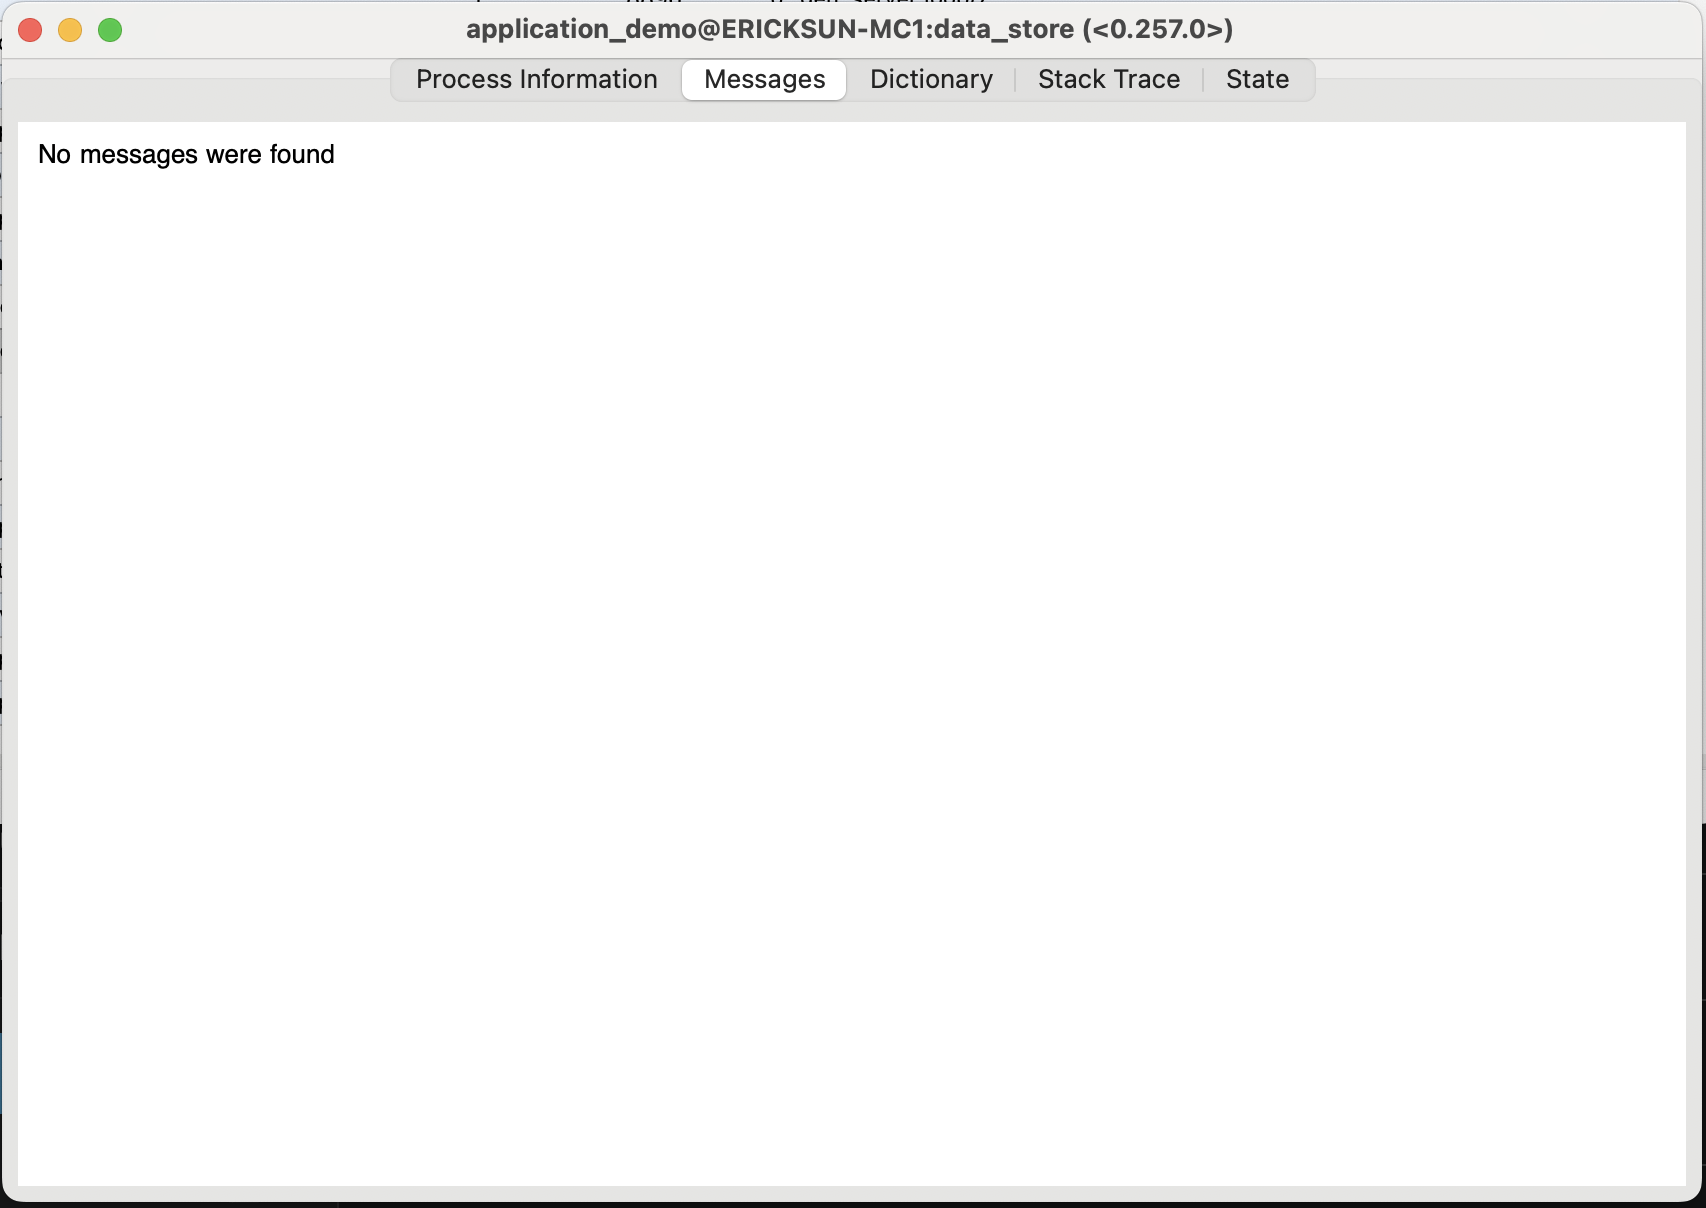
\includegraphics[keepaspectratio]{images/Process_Messages.png}}
\caption{Process Messages}
\end{figure}

\texttt{Messages} tab 对应进程邮箱中尚未处理的消息。它适合和进程列表里的
\texttt{MsgQ} 一起讲：

\begin{Shaded}
\begin{Highlighting}[]
\NormalTok{MsgQ 数值变大}
\NormalTok{  {-}\textgreater{} 说明消息进入速度可能大于处理速度}
\NormalTok{      {-}\textgreater{} 双击进程进入 Messages}
\NormalTok{          {-}\textgreater{} 观察具体积压了哪些消息}
\end{Highlighting}
\end{Shaded}

录课时可以强调：Erlang
进程之间不是共享内存，而是通过消息通信。\texttt{Messages}
页面就是把这种运行时通信方式可视化。

\subsubsection{14.2
Dictionary：观察进程字典}\label{dictionaryux89c2ux5bdfux8fdbux7a0bux5b57ux5178}

\begin{figure}
\centering
\pandocbounded{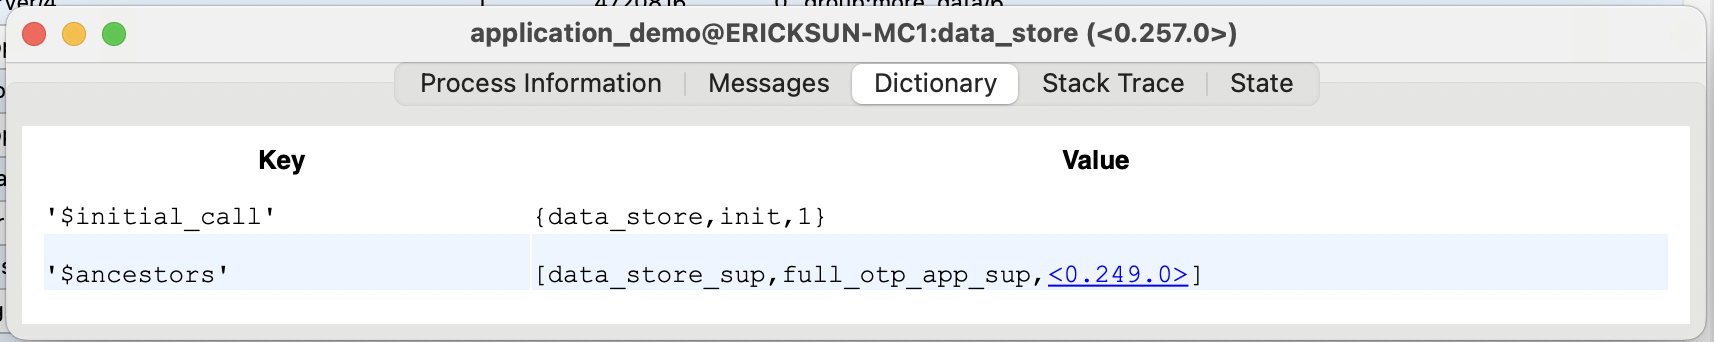
\includegraphics[keepaspectratio]{images/Process_Dictionary.png}}
\caption{Process Dictionary}
\end{figure}

\texttt{Dictionary} tab 展示当前进程的 process dictionary。

进程字典可以理解为``挂在某个进程上的局部键值表''。它有调试价值，但入门课要提醒学习者：普通业务逻辑不要把它当成全局变量或对象字段来滥用，否则代码会变得隐式、难测试。

这一页适合点到为止：知道 Observer
能看到它即可，不建议在前期课程里深入使用。

\subsubsection{14.3 Stack
Trace：观察进程当前调用栈}\label{stack-traceux89c2ux5bdfux8fdbux7a0bux5f53ux524dux8c03ux7528ux6808}

\begin{figure}
\centering
\pandocbounded{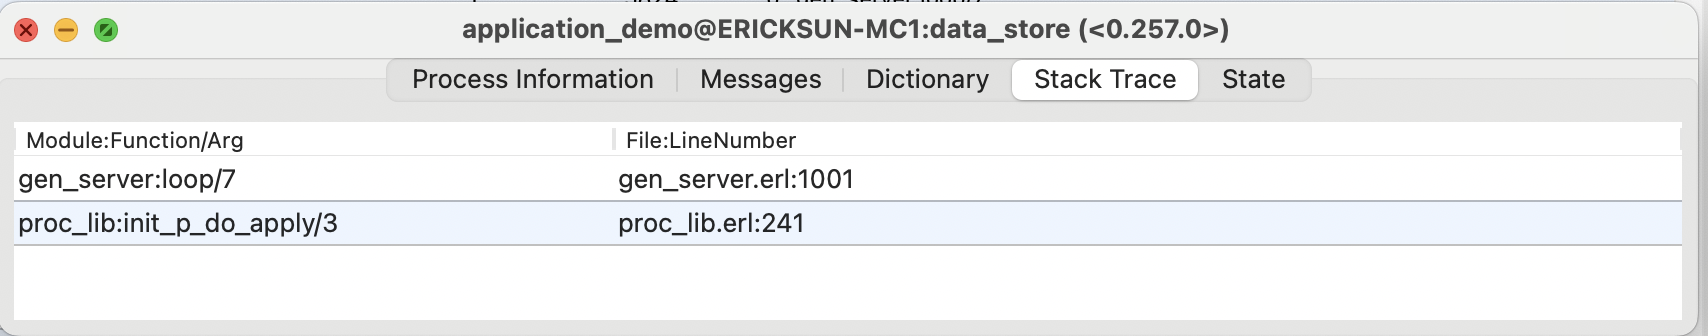
\includegraphics[keepaspectratio]{images/Process_Stack_Trace.png}}
\caption{Process Stack Trace}
\end{figure}

\texttt{Stack\ Trace} tab 用来查看进程当前正在执行的调用路径。

它适合用于这些场景：

\begin{itemize}
\tightlist
\item
  某个进程 CPU 占用异常，想知道它正在跑什么代码。
\item
  某个 \texttt{gen\_server} 响应慢，想判断是否卡在某个函数里。
\item
  教学时说明：BEAM 进程虽然轻量，但仍然是有当前执行栈的运行实体。
\end{itemize}

入门课可以把它和 \texttt{State} 区分开：

\begin{Shaded}
\begin{Highlighting}[]
\NormalTok{State       {-}\textgreater{} 这个 OTP 进程保存了什么业务状态}
\NormalTok{Stack Trace {-}\textgreater{} 这个进程此刻正在执行什么调用路径}
\NormalTok{Messages    {-}\textgreater{} 这个进程还有哪些消息没处理}
\end{Highlighting}
\end{Shaded}

\begin{center}\rule{0.5\linewidth}{0.5pt}\end{center}

\subsection{15. Table Viewer：查看 ETS / DETS
表}\label{table-viewerux67e5ux770b-ets-dets-ux8868}

\begin{figure}
\centering
\pandocbounded{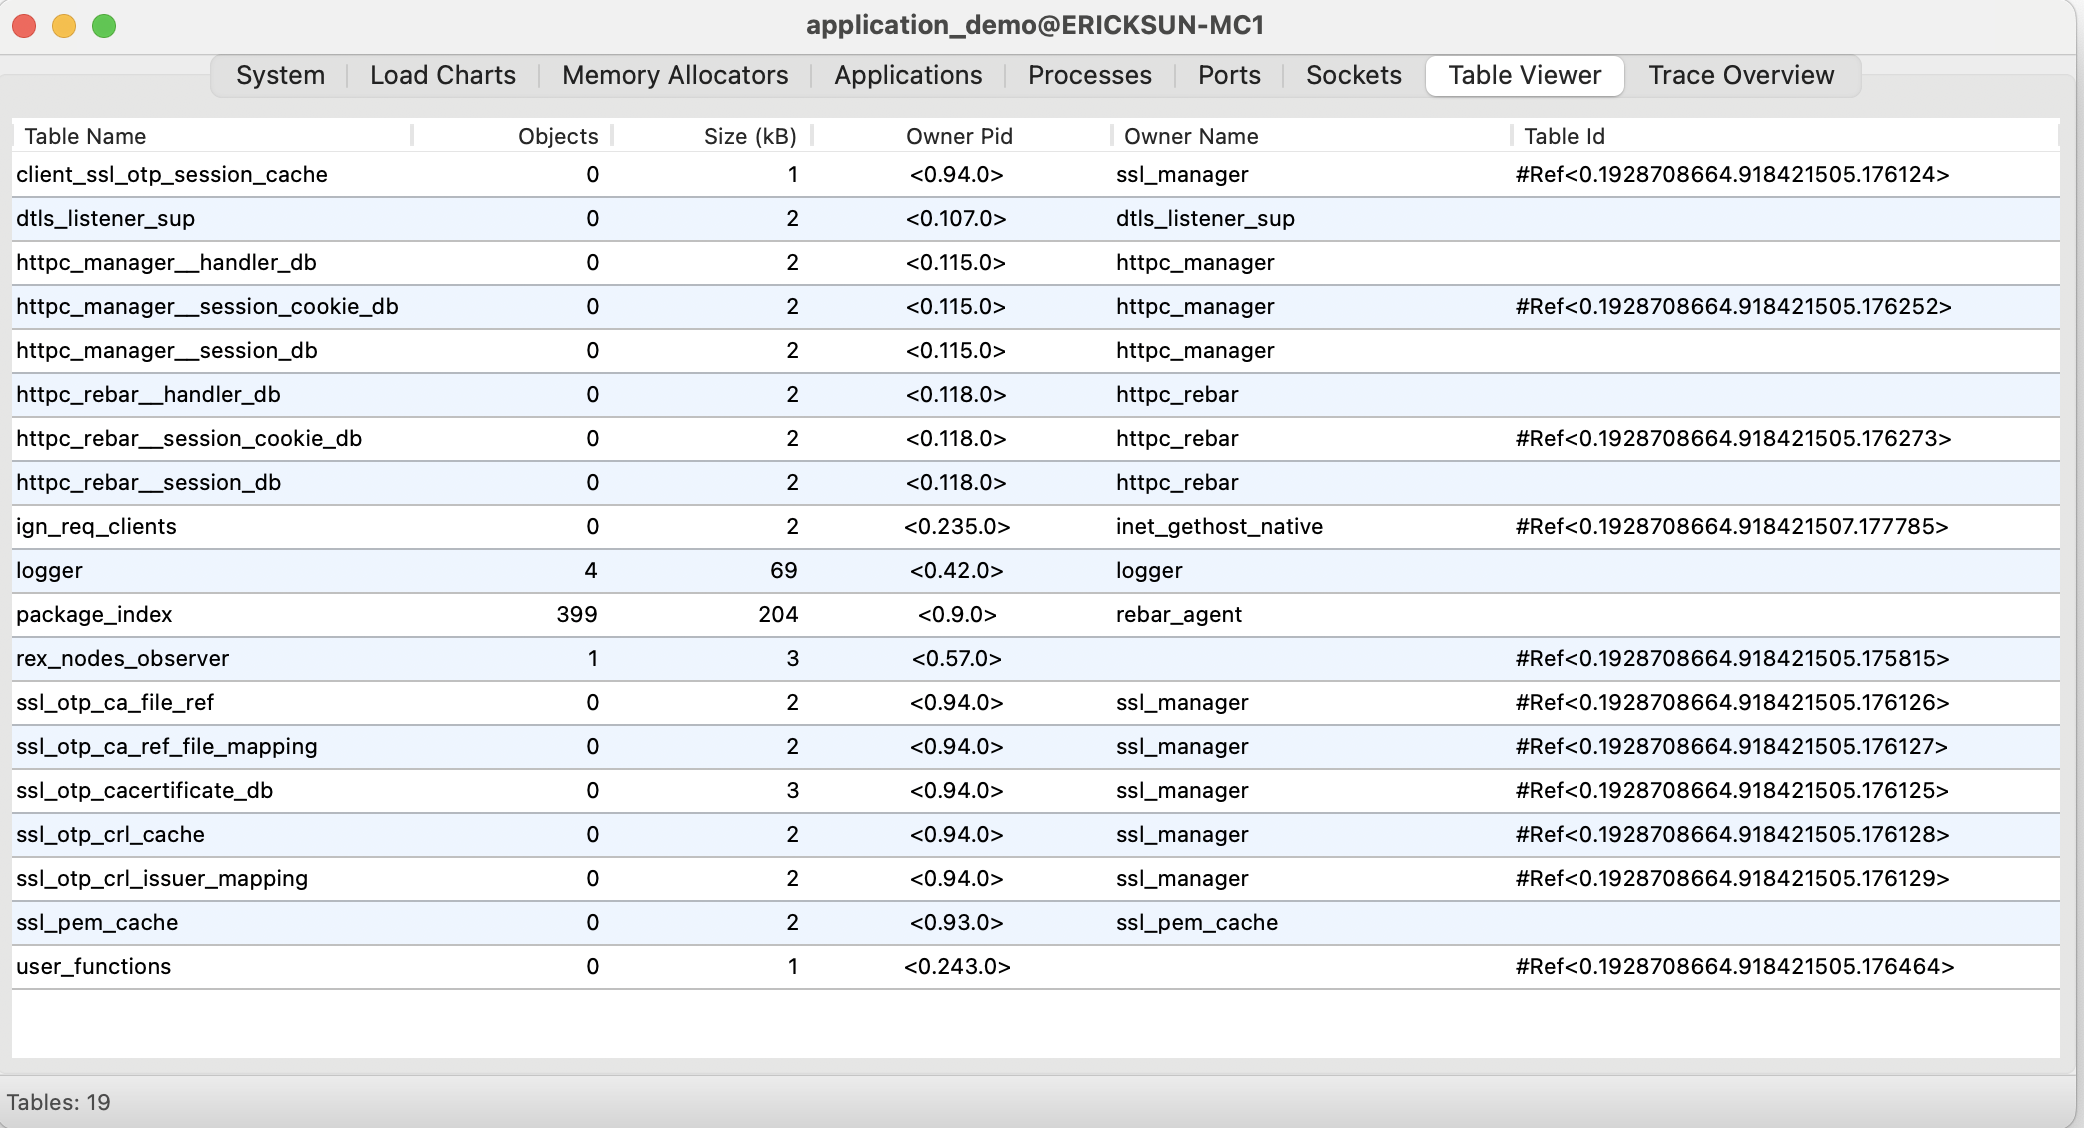
\includegraphics[keepaspectratio]{images/Table_Viewer.png}}
\caption{Table Viewer}
\end{figure}

\texttt{Table\ Viewer} 用来查看节点里的 ETS / DETS 表。对于本 demo
来说，它可以和 \texttt{data\_store} / \texttt{data\_cache} 放在一起讲：

\begin{itemize}
\tightlist
\item
  \texttt{data\_cache} 更适合对应 ETS 这类内存表概念。
\item
  \texttt{data\_store} 更适合对应 DETS 这类磁盘表概念。
\item
  Observer 让``进程状态''和``表数据''可以分开观察。
\end{itemize}

教学时可以这样连接：

\begin{Shaded}
\begin{Highlighting}[]
\NormalTok{Applications / Processes}
\NormalTok{  {-}\textgreater{} 看 OTP 进程结构}

\NormalTok{Process Information / State}
\NormalTok{  {-}\textgreater{} 看某个 gen\_server 的内部状态}

\NormalTok{Table Viewer}
\NormalTok{  {-}\textgreater{} 看节点里的表数据，例如 ETS / DETS}
\end{Highlighting}
\end{Shaded}

这样学习者会更容易理解：OTP
系统不只是一些模块文件，而是由进程、消息、状态、表数据一起组成的运行时系统。

\begin{center}\rule{0.5\linewidth}{0.5pt}\end{center}

\subsection{16. 从 Observer
回到代码}\label{ux4ece-observer-ux56deux5230ux4ee3ux7801}

Observer 不是为了替代代码阅读，而是帮助我们建立代码和运行时之间的映射。

\begin{longtable}[]{@{}
  >{\raggedright\arraybackslash}p{(\linewidth - 2\tabcolsep) * \real{0.6875}}
  >{\raggedright\arraybackslash}p{(\linewidth - 2\tabcolsep) * \real{0.3125}}@{}}
\toprule\noalign{}
\begin{minipage}[b]{\linewidth}\raggedright
Observer 里看到的内容
\end{minipage} & \begin{minipage}[b]{\linewidth}\raggedright
对应代码
\end{minipage} \\
\midrule\noalign{}
\endhead
\bottomrule\noalign{}
\endlastfoot
\texttt{full\_otp\_app} application & \texttt{full\_otp\_app.app.src} 和
\texttt{full\_otp\_app\_app.erl} \\
\texttt{full\_otp\_app\_sup} & \texttt{full\_otp\_app\_sup.erl} \\
\texttt{kv\_server} worker & \texttt{kv\_server.erl} \\
\texttt{traffic\_light} worker & \texttt{traffic\_light.erl} \\
\texttt{data\_store\_sup} 子 supervisor &
\texttt{data\_store\_sup.erl} \\
\texttt{data\_store} / \texttt{data\_cache} & \texttt{data\_store.erl} /
\texttt{data\_cache.erl} \\
Process Information & \texttt{process\_info/1} 能看到的很多信息 \\
State tab & \texttt{sys:get\_state/1} 和 behaviour 内部状态 \\
\end{longtable}

所以本教程后续讲 OTP 时，可以固定使用这个顺序：

\begin{Shaded}
\begin{Highlighting}[]
\NormalTok{先看 Observer 里的现象}
\NormalTok{  {-}\textgreater{} 再看对应源码}
\NormalTok{      {-}\textgreater{} 再回到 Observer 验证运行时变化}
\end{Highlighting}
\end{Shaded}

\begin{center}\rule{0.5\linewidth}{0.5pt}\end{center}

\subsection{17.
课堂演示建议}\label{ux8bfeux5802ux6f14ux793aux5efaux8bae}

建议录课时按这个顺序演示：

\begin{enumerate}
\def\labelenumi{\arabic{enumi}.}
\tightlist
\item
  启动 \texttt{rebar3\ shell\ -\/-sname\ application\_demo}。
\item
  执行 \texttt{observer:start().}。
\item
  看 \texttt{System} 页面，说明 Observer 是节点观察工具。
\item
  切到 \texttt{Applications} 页面。
\item
  先快速看 \texttt{kernel}、\texttt{ssl}、\texttt{inets}。
\item
  选中 \texttt{full\_otp\_app}。
\item
  展开 supervision tree。
\item
  双击 \texttt{full\_otp\_app\_sup}，说明 supervisor 也是进程。
\item
  双击 \texttt{kv\_server}，说明 \texttt{gen\_server} 进程信息。
\item
  切到 \texttt{kv\_server} 的 \texttt{State}，执行
  \texttt{kv\_server:put/2} 后观察状态变化。
\item
  切到
  \texttt{Messages}、\texttt{Dictionary}、\texttt{Stack\ Trace}，说明进程还可以继续向内观察。
\item
  双击 \texttt{traffic\_light}，切到 \texttt{State}，观察
  \texttt{gen\_statem} 当前状态。
\item
  执行 \texttt{traffic\_light:next().}，再观察状态变化。
\item
  打开 \texttt{Table\ Viewer}，说明 ETS / DETS 这类表数据也能在 Observer
  中查看。
\item
  展示 \texttt{Processes} 页面，说明所有进程都在同一个节点里。
\item
  结尾说明：后续会加入 \texttt{observer\_cli}，用于命令行环境观察节点。
\end{enumerate}

\begin{center}\rule{0.5\linewidth}{0.5pt}\end{center}

\subsection{18. Observer 和 observer\_cli
的关系}\label{observer-ux548c-observer_cli-ux7684ux5173ux7cfb}

GUI Observer 适合本地开发、教学录屏和截图讲解；\texttt{observer\_cli}
适合 SSH 到服务器、容器环境或没有图形界面的远程节点。

简单理解：

\begin{Shaded}
\begin{Highlighting}[]
\NormalTok{Observer      {-}\textgreater{} 图形界面，适合讲结构：application / supervisor / worker}
\NormalTok{observer\_cli  {-}\textgreater{} 命令行界面，适合看指标：进程数、内存、reductions、MsgQ、ETS}
\end{Highlighting}
\end{Shaded}

当前 demo 已经在 \texttt{rebar.config} 中加入：

\begin{Shaded}
\begin{Highlighting}[]
\FunctionTok{\{}\CharTok{deps}\FunctionTok{,} \FunctionTok{[}
    \FunctionTok{\{}\CharTok{observer\_cli}\FunctionTok{,} \StringTok{"1.8.8"}\FunctionTok{\},}
    \FunctionTok{\{}\CharTok{recon}\FunctionTok{,} \StringTok{"2.5.6"}\FunctionTok{\}}
\FunctionTok{]\}.}
\end{Highlighting}
\end{Shaded}

\subsubsection{18.1 启动 observer\_cli}\label{ux542fux52a8-observer_cli}

\begin{figure}
\centering
\pandocbounded{
\includegraphics[keepaspectratio]{images/observer_cli_start.png}}
\caption{observer\_cli start}
\end{figure}

在 \texttt{rebar3\ shell} 中启动：

\begin{Shaded}
\begin{Highlighting}[]
\FunctionTok{observer\_cli:start().}
\end{Highlighting}
\end{Shaded}

启动后默认进入 Home 页面。顶部菜单可以看到：

\begin{Shaded}
\begin{Highlighting}[]
\NormalTok{Home(H) | Network(N) | System(S) | Ets(E) | App(A) | Doc(D) | Plugin(P)}
\end{Highlighting}
\end{Shaded}

常用按键：

\begin{longtable}[]{@{}ll@{}}
\toprule\noalign{}
按键 & 用途 \\
\midrule\noalign{}
\endhead
\bottomrule\noalign{}
\endlastfoot
\texttt{H} & 回到 Home 页面 \\
\texttt{A} & 查看 application 聚合信息 \\
\texttt{E} & 查看 ETS 信息 \\
\texttt{S} & 查看系统信息 \\
\texttt{N} & 查看网络信息 \\
\texttt{F} / \texttt{B} & 下一页 / 上一页 \\
\texttt{q} & 退出 \\
\end{longtable}

\subsubsection{18.2 App(A)：查看所有
application}\label{appaux67e5ux770bux6240ux6709-application}

\begin{figure}
\centering
\pandocbounded{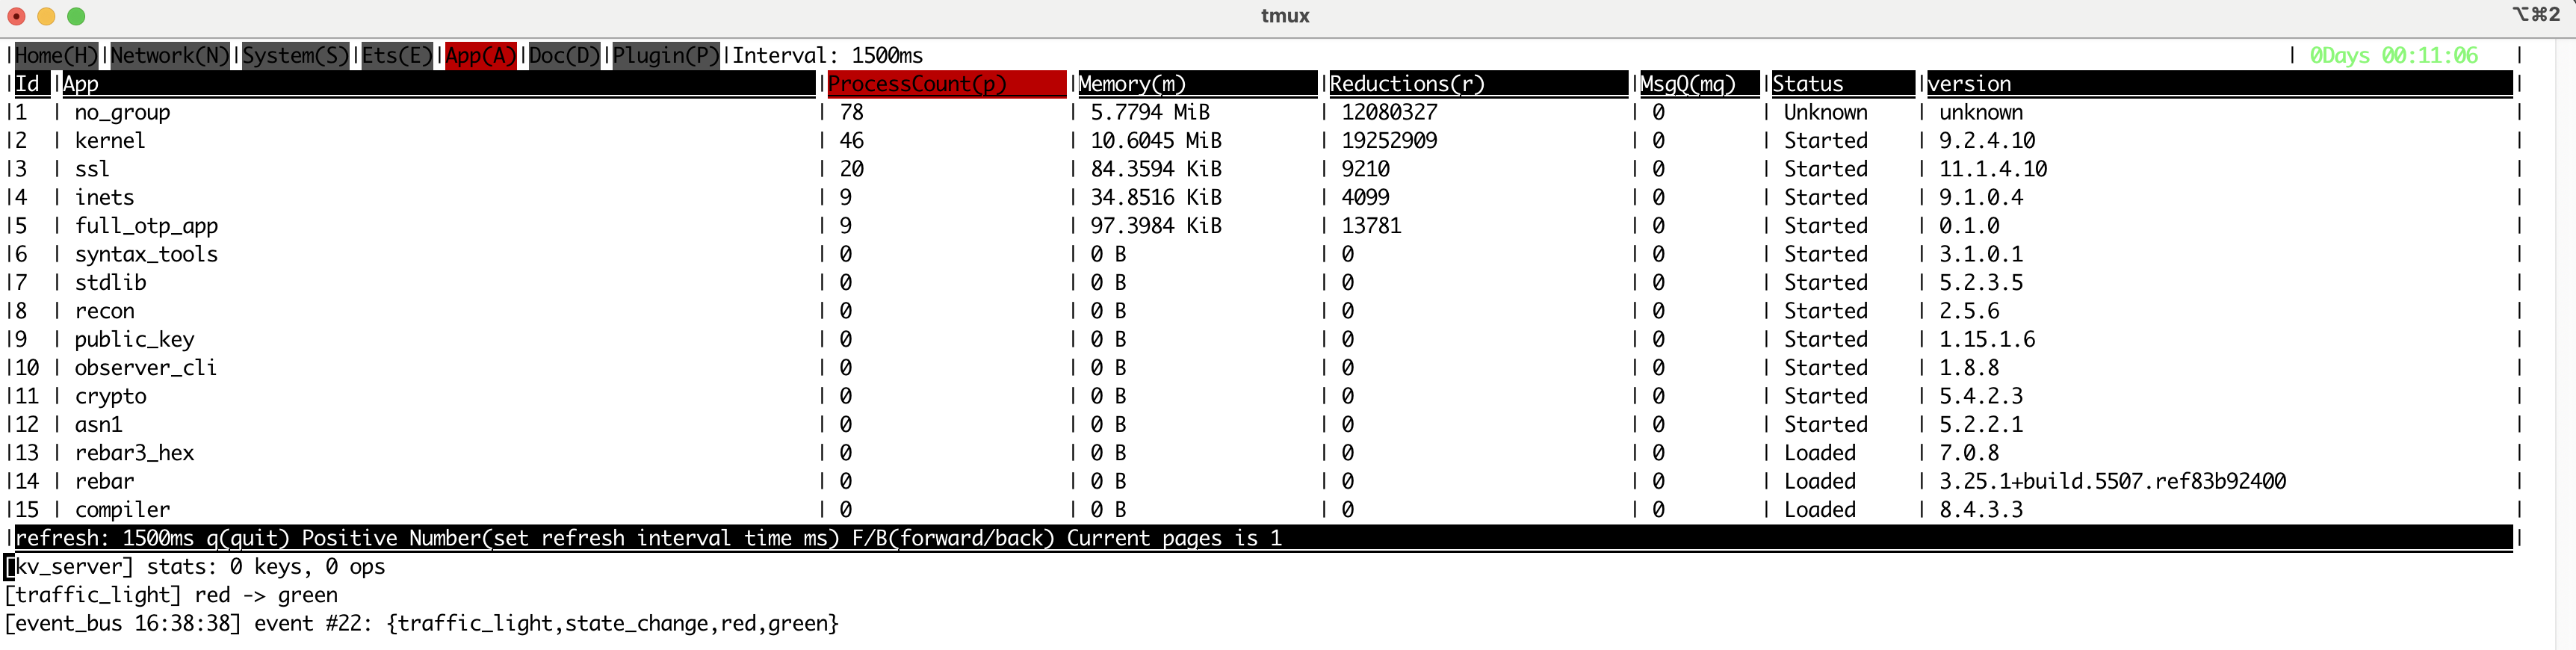
\includegraphics[keepaspectratio]{images/observer_cli_application.png}}
\caption{observer\_cli application}
\end{figure}

按 \texttt{A} 进入 App 页面后，可以看到所有 application 的聚合指标：

\begin{longtable}[]{@{}ll@{}}
\toprule\noalign{}
列 & 含义 \\
\midrule\noalign{}
\endhead
\bottomrule\noalign{}
\endlastfoot
\texttt{App} & application 名称 \\
\texttt{ProcessCount(p)} & 归属到该 application 的进程数量 \\
\texttt{Memory(m)} & 聚合内存占用 \\
\texttt{Reductions(r)} & 聚合 reductions \\
\texttt{MsgQ(mq)} & 聚合消息队列长度 \\
\texttt{Status} & \texttt{Started} / \texttt{Loaded} 等状态 \\
\texttt{version} & application 版本 \\
\end{longtable}

这里可以重点观察 demo 应用：

\begin{Shaded}
\begin{Highlighting}[]
\NormalTok{full\_otp\_app}
\end{Highlighting}
\end{Shaded}

例如截图中 \texttt{full\_otp\_app} 处于 \texttt{Started}
状态，并且能看到进程数量、内存和 reductions。

需要特别说明：\texttt{observer\_cli} 的 App 页面不能像 GUI Observer
那样选中某个 application 后展开 supervisor
tree。这里的行号只是表格编号，不是可进入的菜单项。它适合看 application
资源聚合，不适合讲 supervision tree 结构。

对比关系是：

\begin{Shaded}
\begin{Highlighting}[]
\NormalTok{Observer GUI Applications}
\NormalTok{  {-}\textgreater{} application {-}\textgreater{} supervisor {-}\textgreater{} worker}
\NormalTok{  {-}\textgreater{} 适合讲结构}

\NormalTok{observer\_cli App(A)}
\NormalTok{  {-}\textgreater{} application {-}\textgreater{} ProcessCount / Memory / Reductions / MsgQ}
\NormalTok{  {-}\textgreater{} 适合看资源指标}
\end{Highlighting}
\end{Shaded}

如果要在命令行查看 \texttt{full\_otp\_app} 的监督树，仍然使用 Erlang
shell：

\begin{Shaded}
\begin{Highlighting}[]
\FunctionTok{supervisor:which\_children(}\CharTok{full\_otp\_app\_sup}\FunctionTok{).}
\FunctionTok{supervisor:which\_children(}\CharTok{data\_store\_sup}\FunctionTok{).}
\end{Highlighting}
\end{Shaded}

\subsubsection{18.3
Processes：查看进程列表和进程详情}\label{processesux67e5ux770bux8fdbux7a0bux5217ux8868ux548cux8fdbux7a0bux8be6ux60c5}

\begin{figure}
\centering
\pandocbounded{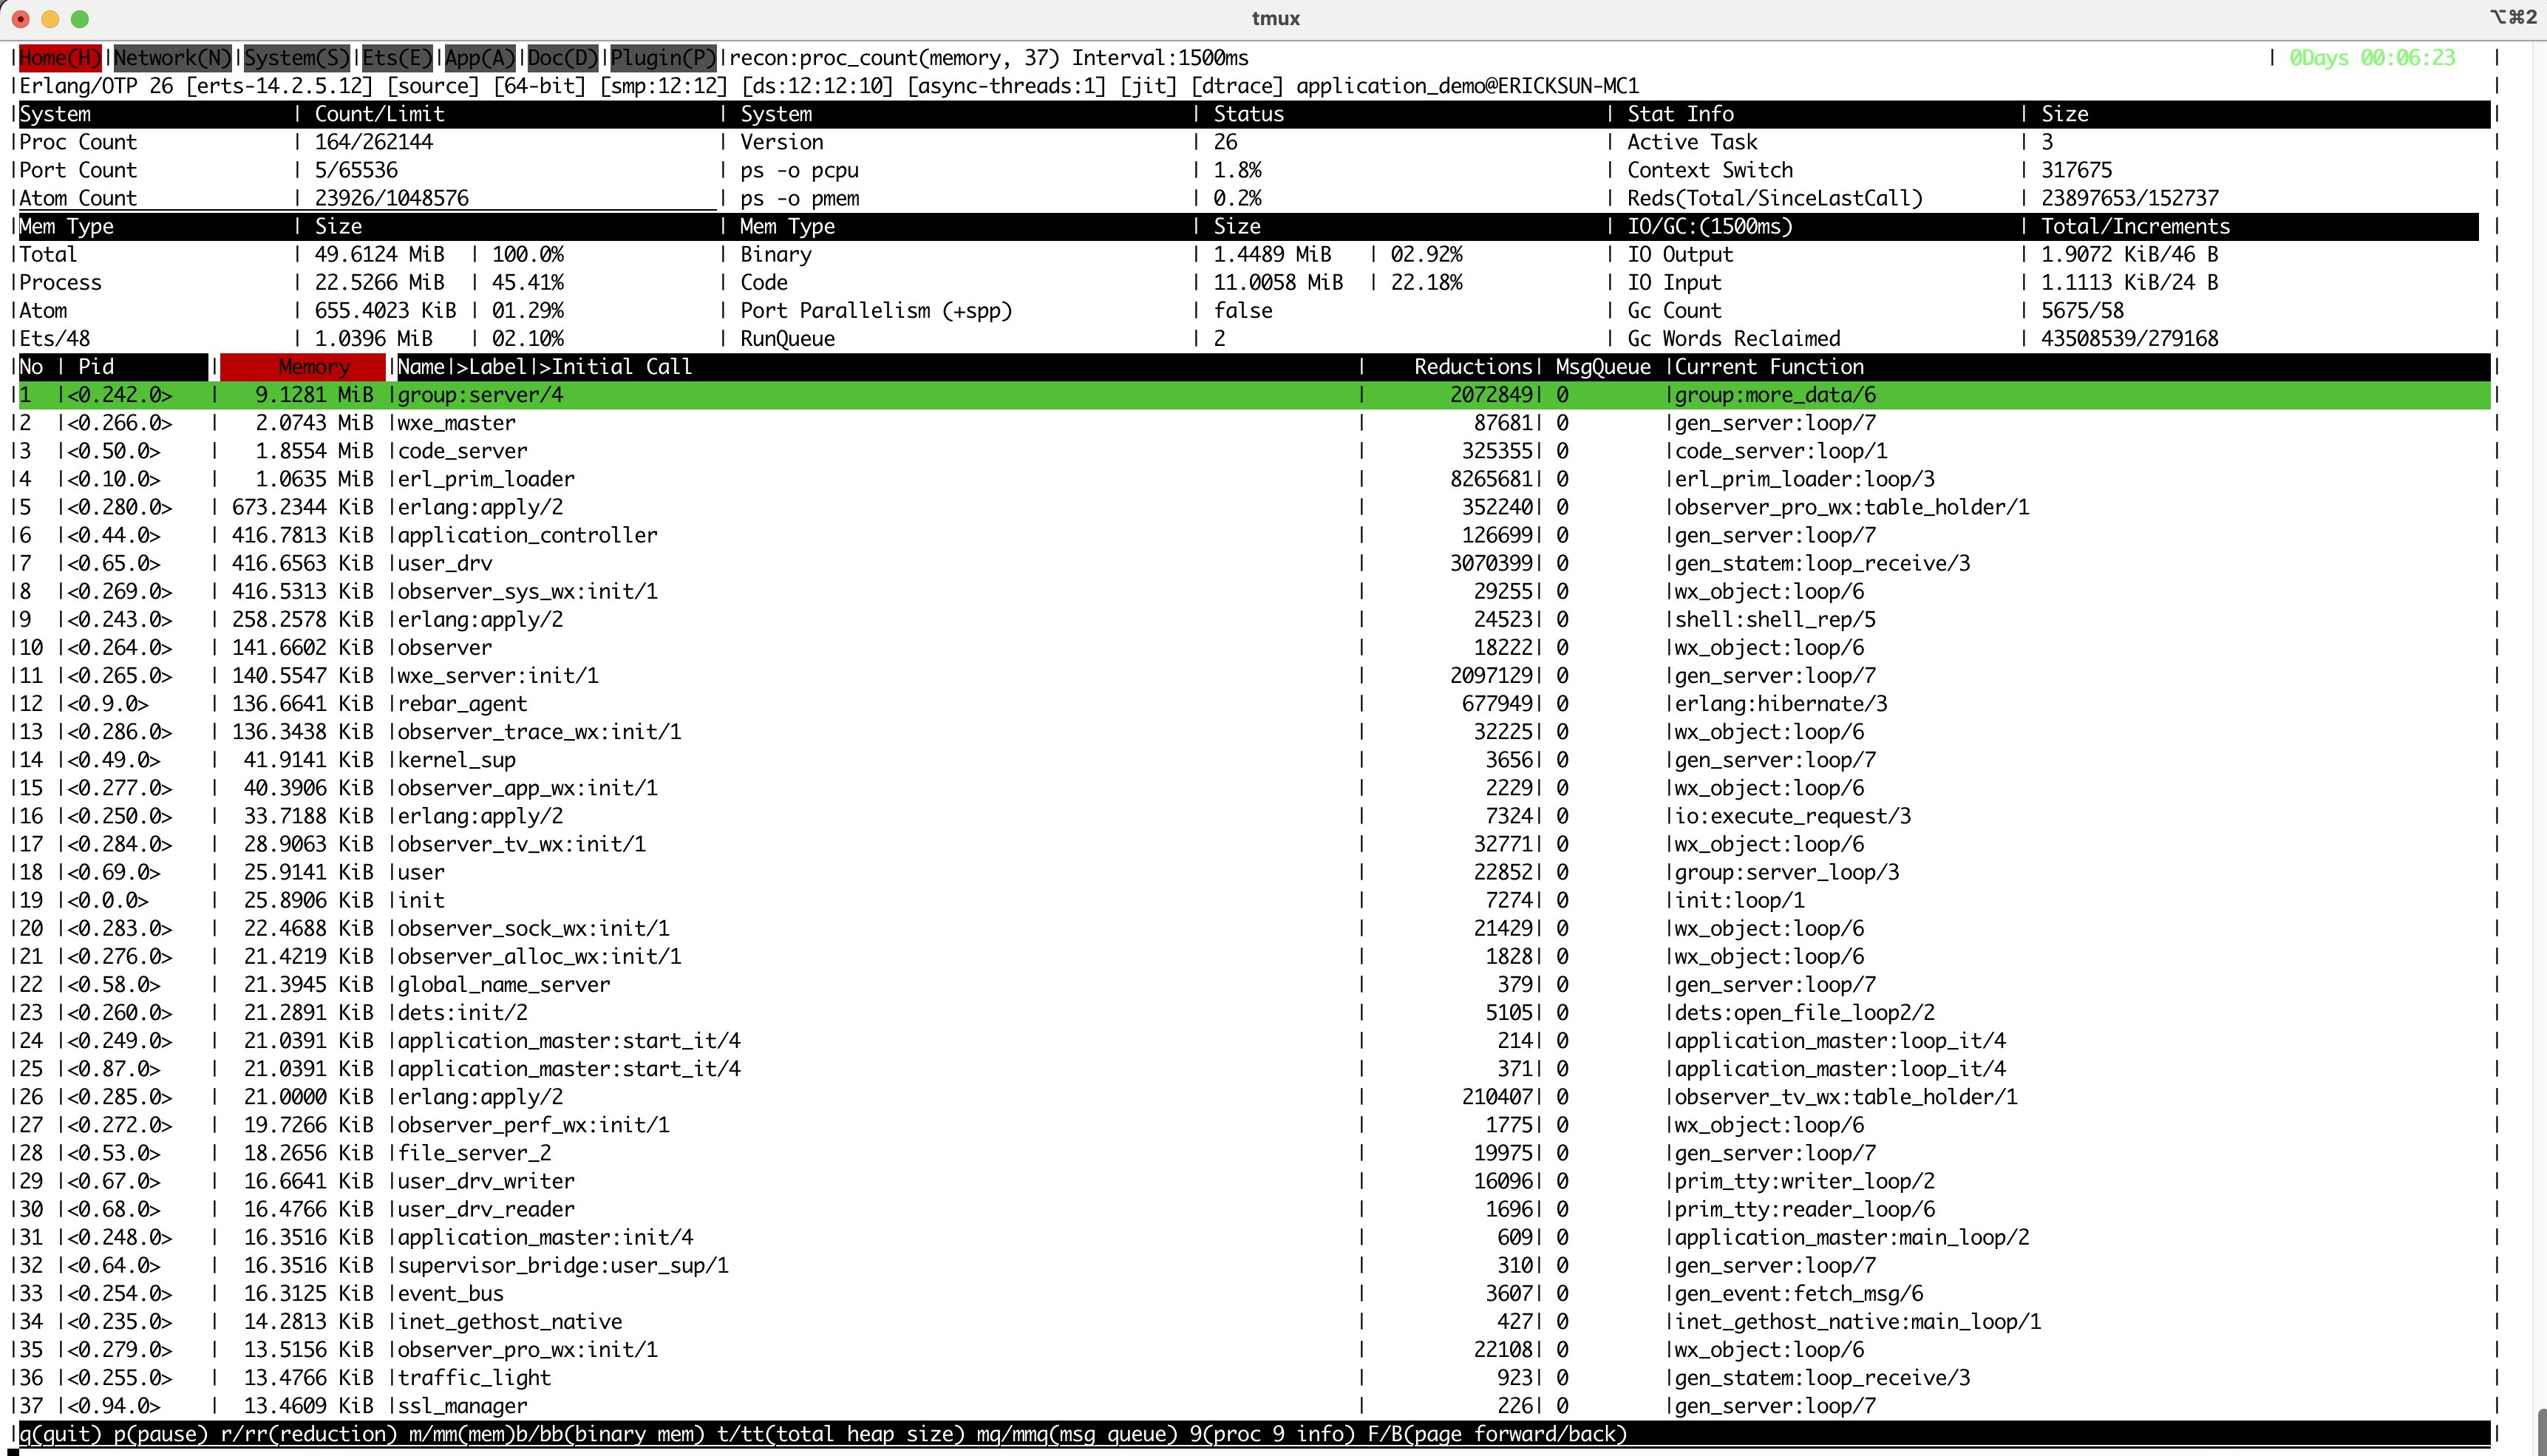
\includegraphics[keepaspectratio]{images/observer_cli_processes.png}}
\caption{observer\_cli processes}
\end{figure}

Home 页面下半部分就是进程列表。它按当前选择的指标排序，例如
memory、reductions、binary memory、message queue。

常用按键：

\begin{longtable}[]{@{}ll@{}}
\toprule\noalign{}
按键 & 用途 \\
\midrule\noalign{}
\endhead
\bottomrule\noalign{}
\endlastfoot
\texttt{m} & 按 memory 排序 \\
\texttt{r} & 按 reductions 排序 \\
\texttt{mq} & 按 message queue 排序 \\
\texttt{F} / \texttt{B} & 下一页 / 上一页 \\
输入进程行号 & 打开该进程详情 \\
\end{longtable}

这一点和 App 页面不同：进程列表中的行号可以进入进程详情，App 页面中的
application 行号不能进入详情。

教学时可以查找这些 demo 进程：

\begin{Shaded}
\begin{Highlighting}[]
\NormalTok{full\_otp\_app\_sup}
\NormalTok{kv\_server}
\NormalTok{event\_bus}
\NormalTok{traffic\_light}
\NormalTok{data\_store\_sup}
\NormalTok{data\_store}
\NormalTok{data\_cache}
\end{Highlighting}
\end{Shaded}

进入进程详情后，可以看到 \texttt{process\_info/2}
能拿到的很多运行时信息，例如 registered name、links、monitors、message
queue、dictionary、current stack 和 state。

\subsubsection{18.4 Ets(E)：查看 ETS
表}\label{etseux67e5ux770b-ets-ux8868}

\begin{figure}
\centering
\pandocbounded{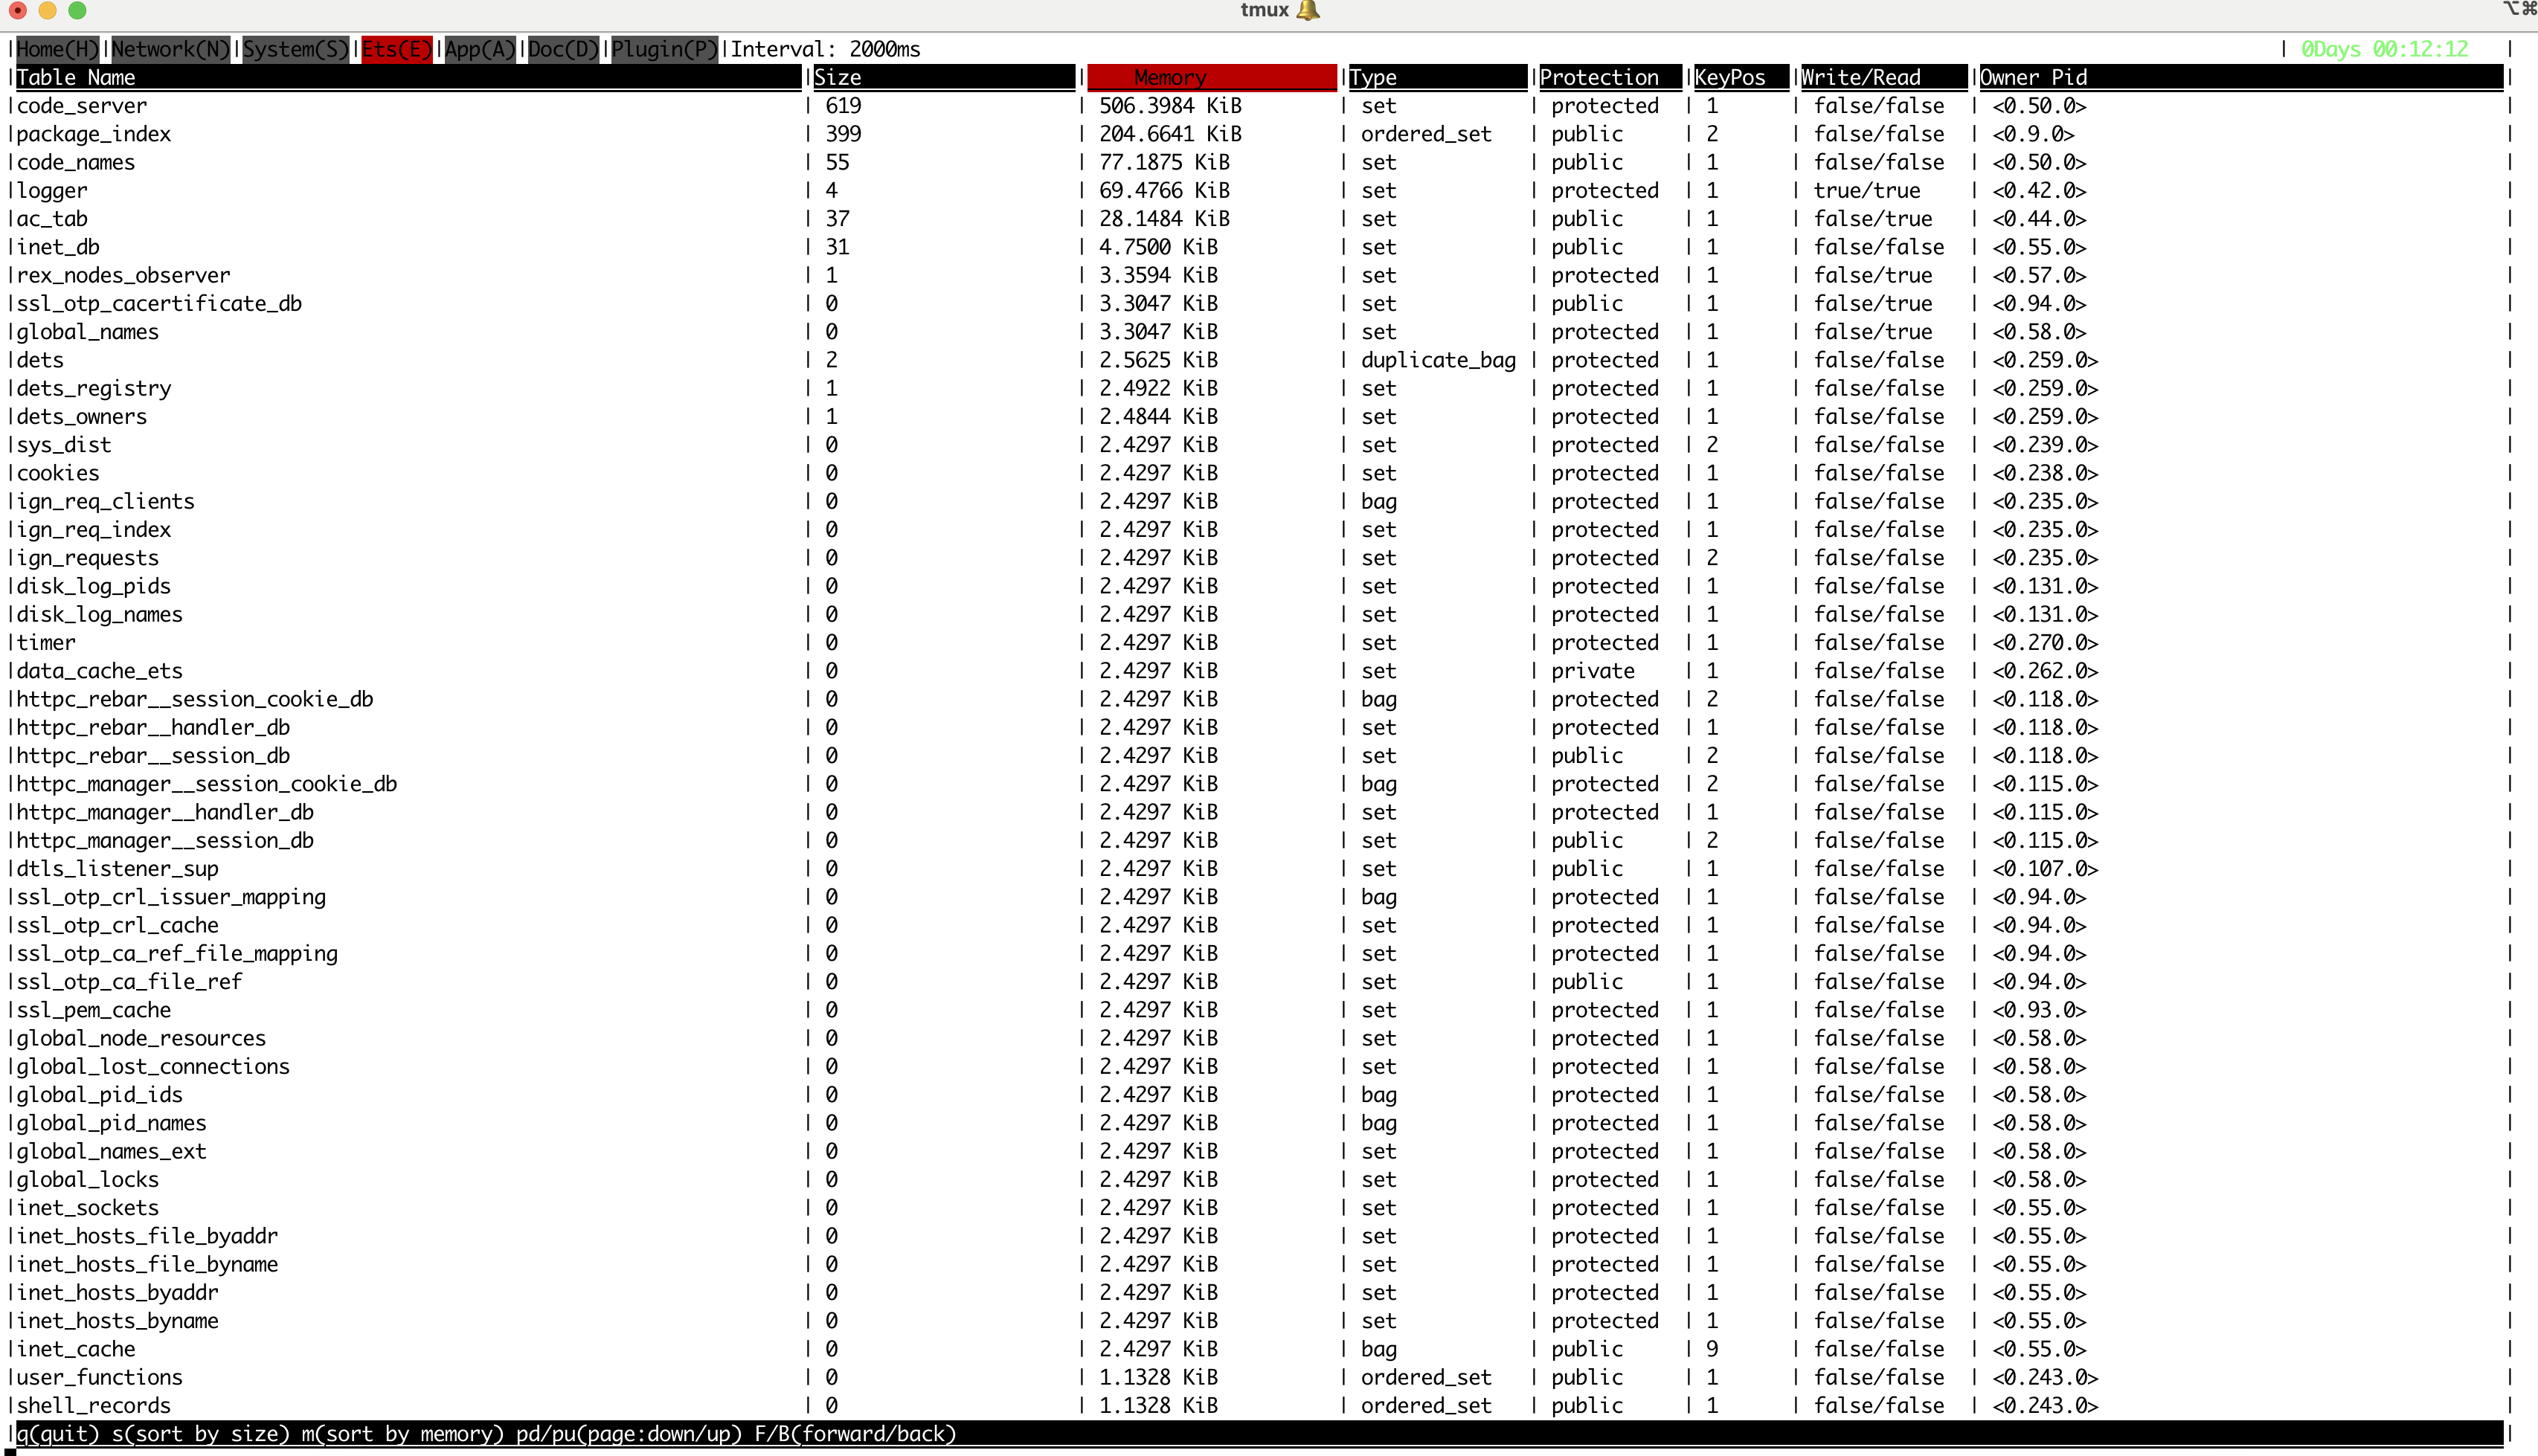
\includegraphics[keepaspectratio]{images/observer_ets.png}}
\caption{observer\_cli ets}
\end{figure}

按 \texttt{E} 可以进入 ETS 页面。它适合和 GUI Observer 的
\texttt{Table\ Viewer} 对比：

\begin{Shaded}
\begin{Highlighting}[]
\NormalTok{GUI Observer Table Viewer}
\NormalTok{  {-}\textgreater{} 图形化查看 ETS / DETS}

\NormalTok{observer\_cli Ets(E)}
\NormalTok{  {-}\textgreater{} 终端中查看 ETS 表指标}
\end{Highlighting}
\end{Shaded}

对于线上排查，\texttt{observer\_cli} 的 ETS
页面更实用，因为它不依赖桌面环境，可以直接在服务器终端里看表数量、表大小和相关指标。

\subsubsection{18.5 用 Erlang API 获取 observer\_cli
类似数据}\label{ux7528-erlang-api-ux83b7ux53d6-observer_cli-ux7c7bux4f3cux6570ux636e}

为了说明 \texttt{observer\_cli} 不是魔法，本 demo 额外提供了一个脚本：

\begin{Shaded}
\begin{Highlighting}[]
\NormalTok{full\_otp\_app/scripts/observer\_cli\_snapshot.escript}
\end{Highlighting}
\end{Shaded}

这个脚本直接调用 Erlang runtime introspection API，采集一次类似
\texttt{observer\_cli}
的快照数据。它的使用方式、参数含义和实现原理已经拆到独立文档：

\begin{Shaded}
\begin{Highlighting}[]
\NormalTok{observer\_cli\_snapshot\_escript.md}
\end{Highlighting}
\end{Shaded}

\begin{center}\rule{0.5\linewidth}{0.5pt}\end{center}

\subsection{19.
当前已有截图清单}\label{ux5f53ux524dux5df2ux6709ux622aux56feux6e05ux5355}

当前 \texttt{images/} 目录已有这些截图，可以支撑本文：

\begin{longtable}[]{@{}
  >{\raggedright\arraybackslash}p{(\linewidth - 2\tabcolsep) * \real{0.5000}}
  >{\raggedright\arraybackslash}p{(\linewidth - 2\tabcolsep) * \real{0.5000}}@{}}
\toprule\noalign{}
\begin{minipage}[b]{\linewidth}\raggedright
图片
\end{minipage} & \begin{minipage}[b]{\linewidth}\raggedright
用途
\end{minipage} \\
\midrule\noalign{}
\endhead
\bottomrule\noalign{}
\endlastfoot
\texttt{observer\_start.png} & 启动 Observer \\
\texttt{System.png} & System 页面 \\
\texttt{Load\_Charts.png} & Load Charts 页面 \\
\texttt{Memory\_Allocators.png} & Memory Allocators 页面 \\
\texttt{Applications.png} & Applications 总览 \\
\texttt{Applications\_kernel.png} & kernel application \\
\texttt{Applications\_ssl.png} & ssl application \\
\texttt{Applications\_inets.png} & inets application \\
\texttt{Applications\_app.png} & full\_otp\_app 总览 \\
\texttt{Applications\_app\_supervisor.png} & full\_otp\_app supervisor
tree \\
\texttt{Applications\_app\_supervisor\_second.png} & 子监督树 \\
\texttt{Applications\_process\_list.png} & Processes 页面 \\
\texttt{Applications\_app\_gen\_server\_process.png} & kv\_server
进程详情 \\
\texttt{Applications\_app\_gen\_server\_state.png} & kv\_server State \\
\texttt{Applications\_app\_gen\_server\_process\_data\_store.png} &
data\_store 进程详情 \\
\texttt{Applications\_app\_gen\_server\_process\_data\_store\_state.png}
& data\_cache/data\_store State \\
\texttt{Applications\_app\_traffic\_light\_process.png} & traffic\_light
进程详情 \\
\texttt{Applications\_app\_traffic\_light\_state.png} & traffic\_light
State \\
\texttt{Process\_Messages.png} & Process Information 的 Messages tab \\
\texttt{Process\_Dictionary.png} & Process Information 的 Dictionary
tab \\
\texttt{Process\_Stack\_Trace.png} & Process Information 的 Stack Trace
tab \\
\texttt{Table\_Viewer.png} & Table Viewer 页面，查看 ETS / DETS
表数据 \\
\texttt{observer\_cli\_start.png} & 启动 observer\_cli \\
\texttt{observer\_cli\_application.png} & observer\_cli 的 App(A)
页面 \\
\texttt{observer\_cli\_processes.png} & observer\_cli 的进程列表 \\
\texttt{observer\_ets.png} & observer\_cli 的 Ets(E) 页面 \\
\end{longtable}

\begin{center}\rule{0.5\linewidth}{0.5pt}\end{center}

\subsection{20.
建议补充截图}\label{ux5efaux8baeux8865ux5145ux622aux56fe}

目前图片已经能完成 Observer GUI 和 \texttt{observer\_cli}
入门讲解。后续如果要继续扩展，可以补充更细的进程详情截图：

\begin{longtable}[]{@{}
  >{\raggedright\arraybackslash}p{(\linewidth - 4\tabcolsep) * \real{0.4286}}
  >{\raggedright\arraybackslash}p{(\linewidth - 4\tabcolsep) * \real{0.3571}}
  >{\raggedright\arraybackslash}p{(\linewidth - 4\tabcolsep) * \real{0.2143}}@{}}
\toprule\noalign{}
\begin{minipage}[b]{\linewidth}\raggedright
建议文件名
\end{minipage} & \begin{minipage}[b]{\linewidth}\raggedright
截图内容
\end{minipage} & \begin{minipage}[b]{\linewidth}\raggedright
用途
\end{minipage} \\
\midrule\noalign{}
\endhead
\bottomrule\noalign{}
\endlastfoot
\texttt{observer\_cli\_process\_info.png} & observer\_cli
中输入进程行号后的进程详情 & 对比 GUI Process Information \\
\texttt{observer\_cli\_system.png} & observer\_cli 的 System(S) 页面 &
对比 GUI System 页面 \\
\texttt{observer\_cli\_network.png} & observer\_cli 的 Network(N) 页面 &
讲远程节点或网络 IO 时使用 \\
\end{longtable}

\begin{center}\rule{0.5\linewidth}{0.5pt}\end{center}

\subsection{21. 小结}\label{ux5c0fux7ed3}

Observer 是学习 Erlang/OTP
的非常重要的入口。它让我们不只是阅读代码，而是直接观察运行中的系统。

本篇最重要的结论是：

\begin{Shaded}
\begin{Highlighting}[]
\NormalTok{application 不是抽象名词，可以在 Observer 里看到。}
\NormalTok{supervisor 不是配置文件，它本身是进程。}
\NormalTok{gen\_server 不是普通对象，它是有 mailbox 和私有状态的 BEAM process。}
\NormalTok{gen\_statem 可以直接显示当前状态机状态。}
\NormalTok{Observer 把 OTP 的运行时结构可视化了。}
\end{Highlighting}
\end{Shaded}

后续讲
\texttt{application}、\texttt{supervisor}、\texttt{gen\_server}、\texttt{gen\_statem}
时，都可以从这篇 Observer 文档开始，把代码和运行时结构连接起来。
